% =====================================================================
%  PROJECT REPORT - FireVLM (Dept. of CSE, Amrita School of Computing, Bengaluru)
%  Compile with XeLaTeX, twice. Keep "amrita_logo.png" in the same folder.
% =====================================================================
\documentclass[12pt]{report}

\usepackage[letterpaper,
            top=1.38in, bottom=1.18in, left=1.58in, right=1.18in,
            headsep=0.38in, footskip=0.5in]{geometry}
\usepackage{fontspec}
\IfFontExistsTF{Times New Roman}{\setmainfont{Times New Roman}}{%
  \IfFontExistsTF{TeX Gyre Termes}{\setmainfont{TeX Gyre Termes}}{%
    \setmainfont{Liberation Serif}}}
\IfFontExistsTF{Calibri}{\newfontfamily\hffont{Calibri}}{%
  \IfFontExistsTF{Carlito}{\newfontfamily\hffont{Carlito}}{%
    \newfontfamily\hffont{Liberation Sans}}}

\usepackage{graphicx}
\usepackage{xcolor}
\usepackage{setspace}
\usepackage{fancyhdr}
\usepackage{titlesec}
\usepackage{titletoc}
\usepackage{enumitem}
\usepackage{array}
\newcolumntype{P}[1]{>{\raggedright\arraybackslash}p{#1}}
\usepackage{booktabs}
\usepackage{amsmath,amssymb}
\usepackage{tikz}
\usetikzlibrary{arrows.meta,positioning,shapes.geometric,calc}
\usepackage{pgfplots}
\pgfplotsset{compat=1.16}
\usepackage[labelsep=colon]{caption}
\usepackage[numbers,square,sort&compress]{natbib}
\usepackage[hidelinks]{hyperref}

\definecolor{wordred}{HTML}{FF0000}
\newcommand{\red}[1]{\textcolor{wordred}{#1}}
\newcommand{\todo}[1]{\textcolor{wordred}{[#1]}}

\setlength{\headheight}{14pt}
\emergencystretch=1em
\setlength{\parindent}{0pt}
\setlength{\parskip}{6pt}


\usepackage{listings}
\usepackage{longtable}
\usepackage{needspace}
\usetikzlibrary{fit,backgrounds,decorations.pathreplacing}
\lstdefinestyle{code}{
  language=Python,
  basicstyle=\ttfamily\footnotesize,
  keywordstyle=\bfseries,
  commentstyle=\itshape\color{gray},
  stringstyle=\color{black},
  columns=fullflexible, keepspaces=true,
  breaklines=true, breakatwhitespace=false, breakindent=0pt,
  postbreak=\mbox{\textcolor{gray}{$\hookrightarrow$}\space},
  frame=single, rulecolor=\color{gray!60}, backgroundcolor=\color{gray!6},
  xleftmargin=4pt, xrightmargin=4pt, framexleftmargin=4pt, framexrightmargin=4pt,
  aboveskip=6pt, belowskip=4pt, showstringspaces=false}
\lstset{style=code}

% ---------------- Details --------------------------------------------
\newcommand{\projecttitle}{FireVLM: Parameter-Efficient Fine-Tuning of a Vision-Language Model for Wildfire Visual Question Answering}
\newcommand{\monthyear}{December 2026}
\newcommand{\guidename}{Dr. Rimjhim Padam Singh, Assistant Professor (Sl.Gd.), Department of Computer Science Engineering}

% ---------------- Headers and footers --------------------------------
\newif\ifinmain
\fancypagestyle{front}{%
  \fancyhf{}
  \renewcommand{\headrulewidth}{0pt}
  \fancyfoot[C]{\thepage}}
\fancypagestyle{main}{%
  \fancyhf{}
  \renewcommand{\headrulewidth}{0pt}
  \fancyhead[L]{\hffont\small\leftmark}
  \fancyhead[R]{\hffont\small\monthyear}
  \fancyfoot[L]{\hffont\small\vspace*{\baselineskip}Dept. of CSE, ASC, Bengaluru}
  \fancyfoot[R]{\hffont\small Page | \thepage\vspace*{\baselineskip}}}
% chapter-opening pages use "plain": same as "main" in the body, page number only in the front matter
\fancypagestyle{plain}{%
  \fancyhf{}
  \renewcommand{\headrulewidth}{0pt}
  \fancyhead[L]{\ifinmain\hffont\small\leftmark\fi}
  \fancyhead[R]{\ifinmain\hffont\small\monthyear\fi}
  \fancyfoot[C]{\ifinmain\else\thepage\fi}
  \fancyfoot[L]{\ifinmain\hffont\small\vspace*{\baselineskip}Dept. of CSE, ASC, Bengaluru\fi}
  \fancyfoot[R]{\ifinmain\hffont\small Page | \thepage\vspace*{\baselineskip}\fi}}
\renewcommand{\chaptermark}[1]{\markboth{#1}{}}
\renewcommand{\sectionmark}[1]{}

\makeatletter
\renewcommand{\chapter}{\global\@topnum\z@\@afterindentfalse
  \secdef\@chapter\@schapter}
\makeatother

\titleformat{\chapter}[display]
  {\normalfont\fontsize{14}{17}\bfseries\centering}
  {CHAPTER - \thechapter}{6pt}{\MakeUppercase}
\titlespacing*{\chapter}{0pt}{0pt}{18pt}
\titleformat{\section}{\normalfont\fontsize{12}{14}\bfseries}{\thesection}{0.6em}{}
\titlespacing*{\section}{0pt}{12pt}{6pt}
\titleformat{\subsection}{\normalfont\fontsize{12}{14}\bfseries}{\thesubsection}{0.6em}{}
\titlespacing*{\subsection}{0pt}{10pt}{4pt}
\setcounter{secnumdepth}{3}
\setcounter{tocdepth}{2}

\contentsmargin{0.5in}
\newcommand{\tocdots}{\titlerule*[0.6pc]{.}}
\titlecontents{chapter}[0pt]{\addvspace{3pt}}
  {CHAPTER \thecontentslabel\ -- \MakeUppercase}
  {\hspace*{0.25in}\MakeUppercase}
  {\tocdots\contentspage}
\titlecontents{section}[0.95in]{}
  {\contentslabel{0.45in}\MakeUppercase}{\MakeUppercase}
  {\tocdots\contentspage}
\titlecontents{subsection}[1.55in]{}
  {\contentslabel{0.6in}\MakeUppercase}{\MakeUppercase}
  {\tocdots\contentspage}
\titlecontents{figure}[0.55in]{\addvspace{2pt}}
  {\contentslabel{0.55in}}{}{\tocdots\contentspage}
\titlecontents{table}[0.55in]{\addvspace{2pt}}
  {\contentslabel{0.55in}}{}{\tocdots\contentspage}

\renewcommand{\contentsname}{TABLE OF CONTENTS}
\renewcommand{\listfigurename}{List Of Figures}
\renewcommand{\listtablename}{List Of Tables}
\renewcommand{\bibname}{REFERENCES}

\captionsetup[figure]{name=Fig., font=bf, labelfont=bf, skip=6pt}
\captionsetup[table]{name=Table, font=bf, labelfont=bf, position=top, skip=6pt}

\renewcommand{\bibnumfmt}[1]{[#1].}
\setlength{\bibsep}{2pt}

\newcommand{\frontchapter}[1]{%
  \clearpage\phantomsection
  \addcontentsline{toc}{chapter}{#1}%
  \chapter*{#1}}

% TikZ styles for diagrams
\tikzset{
  blk/.style={draw, rounded corners=2pt, align=center, minimum height=13mm,
              text width=25mm, font=\footnotesize, fill=gray!8},
  arr/.style={-{Stealth[length=2.2mm]}, thick}
}

\begin{document}
\addtocontents{toc}{\protect\hfill\textbf{Page No.}\protect\par}

% =====================================================================
%  TITLE PAGE
% =====================================================================
\begin{titlepage}
\centering
\vspace*{0.4in}
{\fontsize{14}{17}\selectfont\bfseries \projecttitle\par}
\vspace{10pt}
A PROJECT REPORT\par
\vspace{10pt}
{\fontsize{14}{17}\selectfont\bfseries\itshape Submitted by\par}
\vspace{14pt}
\begin{tabular}{@{}l@{\hspace{0.45in}}l@{}}
BL.EN.U4AIE23123 & Praanesh Balakrishnan Nair\\[16pt]
BL.EN.U4AIE23126 & Rishab Ramesh Nair\\[16pt]
BL.EN.U4AIE23130 & Sanjushree Rajan\\[16pt]
BL.EN.U4AIE23135 & Varun Adhitya G B\\[16pt]
\end{tabular}\par
\vspace{8pt}
{\fontsize{14}{17}\selectfont\bfseries\itshape in partial fulfillment for the award of the degree of\par}
\vspace{12pt}
{\fontsize{14}{17}\selectfont\bfseries BACHELOR OF TECHNOLOGY\par}
\vspace{12pt}
{\small IN\par}
\vspace{14pt}
COMPUTER SCIENCE AND ENGINEERING\par
(Artificial Intelligence) \\
\vspace{10pt}
\IfFileExists{amrita_logo.png}{
\includegraphics[width=1.75in]{amrita_logo.png}}{\todo{amrita\_logo.png not found}}\par
\vspace{10pt}
AMRITA SCHOOL OF COMPUTING, BENGALURU\par
\vspace{10pt}
{\fontsize{14}{17}\selectfont AMRITA VISHWA VIDYAPEETHAM\par}
\vspace{10pt}
BENGALURU 560 035\par
\vspace{10pt}
\MakeUppercase{\monthyear}\par
\end{titlepage}

% =====================================================================
%  FRONT MATTER
% =====================================================================
\pagestyle{front}
\pagenumbering{roman}
\setcounter{page}{1}

\frontchapter{ACKNOWLEDGEMENTS}
\begin{spacing}{1.5}
\setlength{\parindent}{0.5in}
\indent The satisfaction that accompanies successful completion of any task would
be incomplete without mention of people who made it possible, and whose
constant encouragement and guidance have been source of inspiration
throughout the course of this project work.

We offer our sincere pranams at the lotus feet of \textbf{``AMMA'',
MATA AMRITANANDAMAYI DEVI} who showered her blessing upon us throughout the
course of this project work.

We owe our gratitude to \textbf{Prof. Manoj P.}, Director, Amrita Vishwa Vidyapeetham Bengaluru Campus. We would like to place our heartfelt gratitude to \textbf{Dr. Gopalakrishnan E.A.,} Principal, Amrita School of Computing and Amrita School of Artificial Intelligence, Bengaluru for his
valuable support and inspiration.

It is a great pleasure to express our gratitude and indebtedness to our
project guide \textbf{\guidename}, Amrita School of Computing, Bengaluru for
her valuable guidance, encouragement, moral support, and affection
throughout the project work.

We would like to express our gratitude to project panel members for
their suggestions, encouragement, and moral support during the process of
project work and all faculty members for their academic support. Finally,
we are forever grateful to our parents, who have loved, supported and
encouraged us in all our endeavors.
\end{spacing}

\frontchapter{ABSTRACT}
\begin{spacing}{1.5}
Visual Question Answering (VQA) on aerial wildfire imagery enables natural-language querying of active fire scenes using paired visible (RGB) and radiometric thermal inputs. This project investigates parameter-efficient adaptation of vision-language models on the WildFireVQA benchmark using the Sycan Marsh subset (738 image pairs, 34 questions per pair, 25,092 question--answer rows). Two adaptation approaches are examined: a frozen pretrained Qwen2.5-VL-3B-Instruct model evaluated under in-context prompting with zero to ten demonstrations (200 query samples), and compact models combining a frozen CLIP ViT-B/32 encoder, trainable linear projectors, and a 4-bit quantized language model fine-tuned via QLoRA across multiple adapter ranks and target modules. The frozen baseline achieves 15.00\% exact match at zero-shot and 28.00\% at ten-shot. Fine-tuned Qwen2-1.5B models evaluate on 2,482 test queries, achieving 84.13\% to 86.62\% exact match while updating 5.8 to 23.2 million parameters. Configurations adapting query, key, value, and output attention projections at ranks 4 and 8 exhibit performance within sampling uncertainty of each other (86.62\% and 86.30\%), while larger all-linear adapters and higher ranks do not improve accuracy. A Llama-3.2-1B backbone trained under the same pipeline reaches 86.38\% to 88.48\%. The findings indicate that compact attention-only adapter budgets suffice for domain-specific fire-scene visual question answering.
\end{spacing}

\clearpage
{\linespread{0.95}\selectfont\tableofcontents}

\clearpage\phantomsection
\addcontentsline{toc}{chapter}{LIST OF FIGURES}
\listoffigures

\clearpage\phantomsection
\addcontentsline{toc}{chapter}{LIST OF TABLES}
\listoftables

% =====================================================================
%  MAIN CHAPTERS
% =====================================================================
\clearpage
\pagestyle{main}
\inmaintrue
\pagenumbering{arabic}
\setcounter{page}{1}
\onehalfspacing

% ---------------- CHAPTER 1 ------------------------------------------
\chapter{Introduction}

\section{Introduction to Wildfire Visual Question Answering}
Wildfires inflict severe losses on ecosystems, human life, and infrastructure. Aerial surveillance platforms, such as unmanned aerial vehicles (UAVs), capture multimodal visible spectrum (RGB) and radiometric thermal imagery over active fire zones. However, converting these raw sensor streams into actionable situational intelligence---such as identifying active flame fronts, mapping smoke dispersion, and delineating burned perimeters---conventionally relies on manual interpretation by human analysts.

Visual Question Answering (VQA) frames image understanding as natural-language inquiry grounded in visual evidence \cite{antol2015}. Rather than deploying distinct, task-specific classifiers for detection, land-cover categorization, and risk assessment, a VQA interface enables operators to query arbitrary scene properties directly. While modern vision-language models (VLMs) demonstrate strong multimodal comprehension on broad web-scale benchmarks \cite{bai2023,bai2025}, their standard pretraining corpora omit specialized radiometric thermal sensor data. Furthermore, their parameter scale (typically 3 billion to tens of billions of parameters) makes full parameter fine-tuning computationally prohibitive on standard workstation or edge hardware.

This project investigates parameter-efficient adaptation of vision-language models for wildfire visual question answering. Using the WildFireVQA dataset built on the FLAME~3 Sycan Marsh aerial prescribed burn imagery \cite{wildfirevqa,flame3}, we evaluate two adaptation regimes: (i) an in-context learning baseline using a frozen pretrained Qwen2.5-VL-3B-Instruct model prompted with zero to ten demonstrations \cite{brown2020,bai2025}, and (ii) a modular vision-language architecture coupling a frozen CLIP ViT-B/32 vision encoder \cite{radford2021}, dual trainable projection layers, and a 4-bit quantized language model fine-tuned via Low-Rank Adaptation (LoRA/QLoRA) \cite{dettmers2023,hu2022}. The task takes as input a paired aerial RGB image, a radiometric thermal image, and a natural-language query, generating a concise textual answer.

\section{Motivation}
Emergency response agencies require rapid, consistent extraction of information from aerial fire feeds. Full parameter fine-tuning of multi-billion parameter foundation models requires high-memory GPU infrastructure that exceeds the resources of regional monitoring centers and research laboratories. Parameter-efficient fine-tuning via low-rank adapters and 4-bit weight quantization substantially decreases training and memory overhead. However, the extent of adapter capacity required for multimodal disaster question answering remains an open question. This work evaluates how adapter rank and layer placement influence task accuracy and parameter count.

\section{Problem Statement}
Given a paired aerial RGB image, a radiometric thermal image, and a natural-language question, generate the correct concise textual answer while minimizing the number of trainable parameters and operating within the memory constraints of a single commodity GPU.

\section{Objectives}
\begin{itemize}[leftmargin=0.5in, itemsep=2pt]
  \item Establish an audited image-level split with no file overlap between partitions on the Sycan Marsh subset of WildFireVQA \cite{wildfirevqa,flame3}.
  \item Benchmark a frozen pretrained vision-language model across 0-shot to 10-shot in-context demonstrations to assess baseline output formatting and zero-shot reasoning without weight updates.
  \item Construct a modular parameter-efficient vision-language model integrating a frozen CLIP vision encoder, dual trainable modality projectors, and 4-bit quantized language models (Qwen2-1.5B and Llama-3.2-1B) \cite{mithan,llama32}.
  \item Systematically compare adapter placements (attention projections vs.\ all linear projections) and rank sweeps to identify the minimal parameter budget required for fire-scene visual question answering.
\end{itemize}

\section{Organisation of the Report}
The remainder of this report is organized as follows: Chapter~2 surveys related literature in vision-language architectures, parameter-efficient adaptation, and remote sensing. Chapter~3 details software and hardware requirements alongside operational constraints. Chapter~4 presents the architectural design and parameter-efficient configurations. Chapter~5 documents the system implementation and evaluation setup. Chapter~6 describes system testing: the test levels, the data-integrity and model-scoping assertions, the end-to-end checks and the defects they exposed. Chapter~7 analyzes experimental results across models, ranks, and question categories. Finally, Chapter~8 summarizes conclusions and outlines future work.
% src: D-01, D-03, D-04, D-07, DS-001, DS-006, DS-009, DS-012, DS-013, FS-001, FS-002, FS-059, balanced_qkvo_r16-001, qwen2_1_5b_balanced_qkvo_r16-001, balanced_qkvo_r16-018, balanced_qkvo_r16-021

% ---------------- CHAPTER 2 ------------------------------------------
\clearpage
\chapter{Literature Survey}

This chapter reviews the current state of research in vision-language models, parameter-efficient fine-tuning techniques, and their application to specialized domains such as wildfire monitoring. We organize the survey into six key areas: foundations of VLMs and their alignment strategies, parameter-efficient adaptation methods, domain-specific challenges in remote sensing and disaster response, benchmark datasets and model architectures, training data synthesis, and emerging techniques in VLM optimization.

\section{Vision-Language Model Foundations and Alignment}

\subsection{Overview of Vision-Language Models}
Vision-language models have emerged as a transformative approach to bridging visual and textual understanding. A comprehensive survey by researchers across multiple institutions provides a systematic overview of the field, covering pretrained models, fine-tuning strategies, prompt engineering, and adapter mechanisms~\cite{vlmsurvey2024}. The survey identifies three primary architectural paradigms: encoder-decoder models that process vision and language through separate pathways, encoder-only models that fuse modalities early, and decoder-only models that treat visual features as tokens in a unified sequence. The choice of architecture significantly impacts downstream task performance, with decoder-only approaches showing particular promise for generative tasks like VQA.

The evolution of VLMs has been driven by increasingly sophisticated pretraining objectives. Early models relied on contrastive learning between image and text pairs, exemplified by CLIP~\cite{radford2021}, which learns joint embeddings by maximizing agreement between paired image-text representations while minimizing agreement between unpaired ones. Later models incorporated masked language modeling, where random text tokens are masked and predicted from surrounding context and visual features, image-text matching objectives that classify whether an image and caption correspond, and cross-modal reconstruction losses that attempt to reconstruct masked image patches from text descriptions or vice versa. These pretraining strategies learn joint representations that enable zero-shot transfer to novel tasks, though domain-specific adaptation remains necessary for specialized applications.

The survey catalogs major VLM families including CLIP-based models (BLIP, BLIP-2, InstructBLIP), GPT-based models (Flamingo, KOSMOS), and unified architectures (CoCa, BEiT-3). Each family makes different trade-offs between zero-shot generalization, fine-tuning efficiency, and computational cost. The survey also examines benchmark datasets spanning image captioning (COCO Captions, Flickr30K), visual question answering (VQAv2, GQA, OK-VQA), visual reasoning (NLVR2, CLEVR), and multimodal understanding (OKVQA, A-OKVQA), noting that performance on these general-domain benchmarks does not always predict success on specialized tasks like medical imaging or disaster response.

\subsection{Alignment Through Contrastive Learning}
A critical challenge in VLM development is achieving proper alignment between vision and language modalities. Research from Amazon Web Services demonstrates that standard next-token prediction training often results in misaligned embeddings between image and text representations, even after extensive pretraining~\cite{ak2024aligning}. Using t-SNE visualizations of embeddings from models trained with LLaVA's approach, the authors show that image and text embeddings remain disparate in the joint space when trained solely with generative objectives. The visualization reveals distinct clusters for vision and text, with minimal overlap, indicating that the projection module successfully maps images into the language model's token space but fails to ensure semantic alignment.

To address this alignment gap, the authors propose joint training that combines contrastive loss with next-token prediction. The contrastive component explicitly minimizes the distance between matching image-text pairs while maximizing separation between dissimilar pairs, following the InfoNCE loss formulation used in CLIP. Mathematically, for a batch of $N$ image-text pairs, the loss pulls together the embeddings of correct pairs while pushing apart incorrect pairs through a temperature-scaled softmax. This approach achieves approximately 2\% improvement across multiple multimodal benchmarks (MMBench, MME, SEED-Bench, MM-VET, MMMU) without additional computational cost or training data. The method requires only that text embeddings be pre-extracted once during the first training stage, adding negligible overhead.

Crucially, the benefits generalize across different language model backbones (Vicuna-7B, Mistral-7B, Llama3-8B), vision encoders (CLIP ViT variants at different scales), and projection layers (two-layer MLP, C-abstractor with cross-attention, VILA's interleaved pretraining approach, and simple average pooling). Experiments with different vision encoders show that larger models consistently outperform smaller ones: CLIP ViT-L/14-336 achieves 67.2\% on MMBench compared to 55.2\% for ViT-B/32, and higher image resolution (336$\times$336 versus 224$\times$224) provides additional gains by enabling the model to extract finer spatial details.

The work demonstrates that proper alignment in the pretraining stage has downstream benefits that persist through instruction tuning, even though instruction tuning uses only next-token prediction loss. The authors also investigate the role of prompts in contrastive training, finding that carefully designed prompts (``A photo of [caption]'') improve alignment quality for some backbones (Vicuna, Mistral) but not others (Llama3), suggesting that prompt engineering must be tailored to each language model's instruction-following characteristics. The alignment strategy also addresses hallucination in VLMs by ensuring that generated text remains grounded in visual content. Properly aligned embeddings enable the language model to leverage its extensive pretraining on text while maintaining fidelity to the visual input, reducing the tendency to generate plausible but incorrect descriptions.

\section{Parameter-Efficient Fine-Tuning for Vision-Language Models}

\subsection{The Evolution Beyond Transformers}
Parameter-efficient fine-tuning (PEFT) has become essential as VLMs scale to billions of parameters. A recent survey examines PEFT methods specifically for post-Transformer architectures, including Mamba-based state-space models, RWKV recurrent models, and hybrid designs that combine attention with linear-complexity mechanisms~\cite{peft2024survey}. The survey categorizes PEFT approaches into four families: (1) additive methods that insert new trainable modules (adapters, prompt tuning, prefix tuning), (2) selective methods that choose a subset of existing parameters to update while freezing the rest (BitFit, which updates only bias terms; diff pruning, which learns sparse masks), (3) reparameterization methods like LoRA that decompose weight updates into low-rank matrices, and (4) hybrid methods that combine multiple strategies (e.g., MAM Adapter combines LoRA with parallel feed-forward adapters).

For vision-language models, the survey identifies adapter-based methods as particularly effective. Adapters, originally proposed by Houlsby et al.~\cite{houlsby2019}, insert small bottleneck layers between frozen pretrained blocks. A typical adapter has a down-projection from the model dimension $d$ to a smaller bottleneck dimension $d_b$, a nonlinearity (usually GELU or ReLU), and an up-projection back to $d$. The bottleneck creates an information compression that forces the adapter to learn task-specific transformations efficiently. For a model with dimension $d=768$ and bottleneck $d_b=64$, each adapter adds only $2 \times 768 \times 64 \approx 98$K parameters, a tiny fraction of a Transformer block's roughly 3 million parameters.

Prompt tuning, introduced by Lester et al.~\cite{lester2021}, prepends learnable continuous tokens to the input embeddings. Unlike discrete prompt engineering, these ``soft prompts'' are optimized through gradient descent. For VLMs, visual prompt tuning adapts this idea by adding learnable tokens to the vision encoder's input or intermediate layers, effectively programming the encoder to extract task-specific features without modifying its weights. Prefix tuning extends this by adding learnable key and value vectors to each attention layer, giving the model task-specific context at every layer.

Low-rank adaptation (LoRA)~\cite{hu2022} decomposes weight updates into low-rank matrices, dramatically reducing trainable parameters while maintaining expressiveness. For a pretrained weight matrix $W \in \mathbb{R}^{d \times k}$, LoRA keeps $W$ frozen and learns an additive update $\Delta W = BA$, where $B \in \mathbb{R}^{d \times r}$ and $A \in \mathbb{R}^{r \times k}$ with rank $r \ll \min(d,k)$. This reduces trainable parameters from $dk$ to $r(d+k)$. For $d=k=4096$ and $r=8$, the reduction is from 16.8 million parameters to 65K parameters (99.6\% reduction). LoRA's key insight is that task-specific adaptation often lies in a low-dimensional subspace of the full parameter space, so a low-rank update suffices. Empirically, ranks as small as 1–8 often achieve performance close to full fine-tuning on natural language tasks, though vision-language tasks may benefit from slightly higher ranks (4–16) due to the complexity of cross-modal reasoning.

The survey emphasizes that PEFT method choice depends on the target architecture. Mamba models, which replace self-attention with selective state-space layers (linear-time complexity in sequence length), benefit from different adapter placements than Transformers. State-space adapters that modify the continuous-time dynamics of Mamba's hidden state have been proposed, as have hybrid approaches that add small attention layers at key positions. For VLMs combining vision encoders with language models, the optimal strategy often involves freezing the vision encoder entirely (preserving its general visual features) and applying PEFT only to the language component and the projection layer that bridges modalities. This asymmetry reflects the fact that vision encoders like CLIP are pretrained on massive image-text datasets (400M–2B samples) and transfer well, whereas language models benefit from task-specific adaptation to interpret visual features in the target domain.

\subsection{Adaptive Parameter Selection}
While PEFT methods reduce trainable parameters, selecting which parameters to adapt remains challenging. Research on adaptive parameter selection proposes dynamic strategies that identify the most important parameters for a given task~\cite{adaptive2024}. Rather than applying uniform adapter ranks or selecting layers manually, adaptive methods use gradient information, sensitivity analysis, or learned gating mechanisms to allocate capacity where it provides maximum benefit.

The paper introduces a meta-learning framework that treats parameter selection as a discrete optimization problem. Given a budget of trainable parameters, the method searches over candidate configurations (which layers receive adapters, what rank for each adapter, whether to include prompt tuning) and estimates each configuration's performance using a small validation set. The search uses gradient-based meta-learning or evolutionary algorithms to efficiently explore the combinatorial space. Once a configuration is selected, the model is trained on the full dataset with that configuration fixed.

Experiments on vision-language benchmarks show that adaptive selection outperforms uniform allocation. For example, with a budget of 5 million trainable parameters on a 7B-parameter VLM, uniform LoRA with rank 8 across all layers achieves 72.3\% accuracy on a visual reasoning task, whereas adaptive selection (rank 16 on cross-attention layers, rank 4 on self-attention layers, no adapters on early vision layers) achieves 75.1\%. The adaptive method identifies that cross-modal fusion layers benefit most from higher capacity, while early vision processing and late language generation require minimal adaptation.

For vision-language tasks, adaptive selection can focus capacity on layers that handle cross-modal reasoning (the projection layer and the first few language model layers that process visual tokens) while using minimal parameters for modality-specific processing deeper in the language model. This approach is particularly valuable when computational budgets are constrained, as in edge deployment or when training on limited hardware. The method also discovers task-specific patterns: visual reasoning tasks benefit from adapters in attention layers, while image captioning benefits more from adapters in feed-forward layers that generate fluent text. This insight suggests that different VQA subtasks (counting, spatial reasoning, attribute recognition) may require different adapter configurations for optimal efficiency.

\subsection{Knowledge-Decoupled Adapter Tuning}
Knowledge-decoupled adapter (KDA) tuning addresses a key limitation of standard adapters: they conflate task-specific adaptation with preservation of pretrained knowledge~\cite{kda2024}. KDA separates these objectives by introducing parallel adapter paths—one for general knowledge retention and another for task-specific learning. This architecture allows the model to maintain strong zero-shot capabilities on held-out domains while specializing for the target task.

The KDA architecture consists of two branches at each adapted layer. The knowledge-preservation branch uses fixed or lightly regularized adapters that maintain the model's original capabilities, while the task-specific branch learns freely to optimize performance on the target task. The outputs of both branches are combined through a learned gating mechanism that dynamically balances general and specific knowledge based on the input. During training, the knowledge-preservation branch is trained with a distillation loss that encourages it to match the pretrained model's outputs, while the task-specific branch optimizes task performance. This dual-objective training prevents catastrophic forgetting while enabling strong adaptation.

Experiments on vision-language benchmarks demonstrate KDA's effectiveness. On a medical VQA task, standard LoRA achieves 78.3\% in-domain accuracy but drops to 52.1\% on general visual reasoning questions, indicating severe forgetting. KDA achieves 76.8\% in-domain accuracy (slightly lower) but maintains 68.4\% on general reasoning (dramatically better), demonstrating successful knowledge preservation. The method also improves few-shot learning: when presented with examples from a new domain during inference, KDA adapts more quickly than standard adapters because its general knowledge branch provides a strong foundation for transfer.

For VLMs, KDA is especially relevant when adapting general-purpose models to specialized domains like medical imaging, remote sensing, or disaster response. The decoupled design ensures that domain adaptation does not catastrophically forget general visual reasoning abilities, enabling the model to handle both in-domain queries (``Is there active fire in this thermal image?'') and unexpected out-of-domain questions (``What type of terrain is shown?''). This robustness is critical for safety-critical applications where the model may encounter diverse queries during deployment.

\subsection{Granularity Control with VL-PET}
VL-PET (Vision-Language Parameter-Efficient Tuning) introduces granularity control, allowing practitioners to tune the balance between parameter efficiency and model expressiveness~\cite{vlpet2024}. The method parameterizes PEFT strategies along a continuum from extremely sparse (updating less than 0.1\% of parameters) to moderately sparse (1-5\% of parameters), with corresponding trade-offs in adaptation quality. This flexibility is achieved through a unified framework that encompasses multiple PEFT techniques and controls their capacity through a single granularity parameter.

VL-PET achieves granularity control through hierarchical adapter structures and dynamic rank allocation. At the coarsest granularity level, the method applies low-rank adapters ($r=1$ or $r=2$) to only the final layers of the language model, capturing high-level task structure with fewer than 100K trainable parameters. At intermediate granularity, adapters with moderate rank ($r=4$ to $r=8$) are added to more layers, including cross-attention modules that fuse vision and language. At the finest granularity, higher-rank adapters ($r=16$ or $r=32$) span all attention and feed-forward layers, approaching the expressiveness of full fine-tuning while still using only 1-5\% of total parameters.

The framework includes automated search over granularity configurations using a performance predictor. Given a validation set and a parameter budget, the predictor estimates accuracy for candidate configurations without full training, using features like layer depth, adapter placement, and rank. This enables efficient architecture search that identifies optimal points on the accuracy--efficiency frontier. Experiments show that the optimal granularity is task-dependent: simple tasks like binary classification achieve 95\% of full fine-tuning performance with 0.1\% parameters, while complex reasoning tasks require 1-2\% parameters to reach the same relative performance.

VL-PET also introduces a progressive training schedule that begins with coarse granularity and gradually increases adapter capacity during training. This curriculum approach improves final accuracy compared to training at fixed granularity, as early training with sparse adapters acts as regularization that prevents overfitting, while later training with denser adapters enables the model to learn complex patterns. This capability is crucial for scenarios where memory and compute budgets vary. A deployment on a high-end server might use fine-grained adaptation for maximum accuracy, while a mobile deployment uses coarse-grained adaptation for acceptable performance within tight constraints. For wildfire VQA, this flexibility allows experimentation with different granularity levels to find the optimal trade-off between accuracy and training cost on free-tier GPUs.

\section{Vision-Language Models in Remote Sensing and Disaster Response}

\subsection{Remote Sensing with VLMs}
Remote sensing presents unique challenges for VLMs: high-resolution imagery with fine spatial detail, multi-spectral data beyond RGB (thermal, hyperspectral, SAR), geospatial reasoning requirements, and limited annotated training data. A comprehensive survey on vision-language modeling for remote sensing~\cite{remotesensing2024} catalogs existing datasets, model architectures, and domain-specific adaptations.

The survey identifies key differences between natural images and remote sensing data. Satellite and aerial images often have resolution exceeding $10,000 \times 10,000$ pixels, requiring efficient patch-based processing. Objects of interest (vehicles, buildings, fires) may occupy only a small fraction of the frame, demanding strong spatial reasoning and attention mechanisms. Multi-spectral data requires fusion strategies that preserve information from each band while learning cross-spectral relationships.

Current remote sensing VLMs adapt pretrained models through specialized pretraining on geo-tagged image-caption pairs, architectural modifications to handle high-resolution input, and task-specific fine-tuning for applications like land-cover classification, change detection, and disaster assessment. The survey highlights the need for more diverse benchmarks covering different sensor modalities, geographic regions, and temporal scales.

\subsection{Wildfire Visual Question Answering}
The WildFireVQA benchmark~\cite{wildfirevqa} addresses a critical gap in disaster response VLMs. Created by researchers at Clemson University, the dataset contains 6,097 RGB-thermal image pairs from three prescribed burns (Sycan Marsh, Willamette, Shoetank) captured by the FLAME~3 project~\cite{flame3}. Each image pair is annotated with 34 questions spanning six categories: presence and detection (is there fire?), counting (how many hotspots?), spatial reasoning (where is the smoke relative to the flame?), scene understanding (what is the dominant vegetation?), temperature analysis (what is the maximum temperature?), and comparative reasoning (which area is hotter?). This yields 207,298 total question-answer pairs.

The dataset uses radiometric thermal TIFFs that encode per-pixel temperature measurements, not just visual thermal colorization. This enables temperature-based reasoning impossible with RGB-only data. Questions were generated by GPT-4o and validated by wildfire experts to ensure realism and correctness. The benchmark evaluates models in multiple-choice format with four options per question.

Baseline results reveal significant challenges. General-purpose VLMs like BLIP-2, InstructBLIP, LLaVA-1.5, and Qwen-VL achieve only 26.4--36.5\% accuracy when trained on remote sensing data, barely exceeding random chance (25\%). Even GPT-4o, the strongest baseline, reaches only 75.0\% test accuracy. Performance varies sharply by question category: GPT-4o achieves 81\% on scene understanding but only 41\% on counting and 44\% on temperature analysis. This suggests that current VLMs lack robust thermal reasoning and fine-grained spatial understanding required for wildfire monitoring.

The WildFireVQA paper emphasizes that the benchmark enables evaluation of models on safety-critical real-world tasks where errors have consequences. Deploying VLMs for fire response requires accuracy exceeding 90\%, particularly on presence detection and spatial reasoning categories that inform evacuation and resource deployment decisions.

\subsection{UAV-Based Wildfire Detection Systems}
Beyond VQA benchmarks, practical wildfire systems integrate VLMs with autonomous platforms. A recent framework~\cite{uavwildfire2024} proposes using UAV swarms with spiral coverage algorithms to monitor forests, analyzing captured imagery with VLMs to detect early fire indicators (light smoke, vegetation discoloration, thermal anomalies), and deploying fire-retardant foam via fast-response drones when hazards are identified. This end-to-end system combines sensing (UAV swarm), fog computing (local VLM inference at ground stations), cloud storage (historical data and model retraining), and application services (crowdsourcing and decision dashboards).

The VLM component uses vision-language understanding to distinguish true fire signatures from visual confusers like sunsets and red skies, achieving over 99\% detection accuracy on a specialized fire-detection dataset. Semantic understanding enables the system to reason about context (``Is this smoke from a fire or morning fog?'') rather than relying solely on pixel-level pattern matching. The framework shifts wildfire management from reactive response to proactive prevention, addressing fires before full ignition.

This work demonstrates that VLMs trained for wildfire VQA can transfer to operational systems when paired with appropriate sensing and actuation infrastructure. The ability to answer natural-language queries (``Where is the fire spreading?'' ``Should we evacuate this area?'') provides flexibility that fixed classifiers cannot match.

\section{Model Architectures and Training Paradigms}

\subsection{Open-Weight Vision-Language Models}
Molmo and PixMo, developed by the Allen Institute for AI, represent state-of-the-art open-weight VLMs~\cite{molmo2024}. Molmo models achieve performance competitive with proprietary systems like GPT-4V and Claude 3.5 Sonnet while releasing full weights, training data, and training code under permissive licenses. The family includes Molmo-72B (72 billion parameters, based on Qwen2-72B), Molmo-7B-D (7 billion parameters with dense architecture based on Qwen2-7B), Molmo-7B-O (7B with OLMo language model), and MolmoE-1B (1 billion parameters with mixture-of-experts architecture). All variants use a frozen ViT-L/14 CLIP vision encoder (336$\times$336 resolution) or SigLIP encoder, a trainable multi-layer perceptron connector module that projects vision features into the language model's embedding space, and a decoder-only language model.

The key innovation is PixMo, a carefully curated dataset of 1.1 million image-text pairs combining human annotations from expert annotators, synthetic captions from strong teacher models (GPT-4V, Gemini 1.5), and carefully filtered academic datasets with permissive licenses (COCO, Visual Genome, AI2D science diagrams). PixMo emphasizes pointing and counting tasks, which are underrepresented in existing VLM training data but critical for spatial reasoning. The dataset includes detailed object descriptions with fine-grained attributes, spatial relationships expressed in natural language (``the red car to the left of the building''), and numerical reasoning examples that require counting discrete objects or comparing quantities. Unlike web-scraped datasets, every PixMo sample underwent human verification to ensure accuracy, removing noisy or incorrect annotations that degrade model quality.

Molmo's training procedure uses a three-stage pipeline: (1) connector pretraining on large-scale image-caption pairs (LAION subsets, DataComp) to learn basic vision-language alignment, (2) mid-stage training on PixMo to develop core VLM capabilities including pointing (identifying object locations via coordinate prediction), counting, detailed captioning, and visual reasoning, and (3) final fine-tuning on high-quality instruction data (LLaVA-Instruct filtered for quality) to improve instruction-following and conversational ability. This progression from broad to narrow tasks mirrors curriculum learning in humans, where general skills are acquired before specialization. The language model backbone remains frozen during stages 1 and 2, with only the connector trainable, and is unfrozen in stage 3 for full model fine-tuning.

Results show that data quality dominates data scale for VLM training. Molmo-7B-D trained on 1.1M carefully curated PixMo samples achieves 81.4\% on MMBench and 73.2\% on SEED-Bench, outperforming models trained on 100M+ noisier web-scraped pairs (e.g., LLaVA-1.5-7B achieves 64.8\% and 60.4\% respectively on the same benchmarks). Molmo-72B reaches 82.3\% on MMBench, competitive with GPT-4V (81.7\%), despite using a fraction of the training data. Ablations show that removing human annotations from PixMo drops performance by 5-8 points, confirming the value of expert curation.

For practitioners, Molmo provides strong open baselines. The 7B and 1B variants are feasible to fine-tune with PEFT on academic hardware (the 7B model with 4-bit quantization and LoRA adapters fits on a single 24GB GPU), and the released code includes examples of adapter-based domain adaptation. The permissive licensing enables commercial use and derivative work, unlike many academic VLMs that restrict commercial deployment.

\subsection{Spatial Reasoning with VisionCore}
Spatial reasoning—understanding object locations, sizes, relative positions, and spatial relationships—is essential for VQA but poorly addressed by standard VLMs~\cite{visioncore2024}. VisionCore introduces architectural modifications that enhance spatial reasoning without sacrificing general vision-language performance. The model augments CLIP-style vision encoders with explicit spatial embeddings that encode absolute patch positions (2D coordinates normalized to $[0,1]$) and relative geometric relationships between patches (Euclidean distance, angular direction, and inclusion relationships for nested regions).

The spatial embeddings are learned through a dedicated pretraining task where the model must predict spatial relationships from natural language descriptions. For example, given an image and the text ``the car is to the left of the building,'' the model learns to identify the car's patch, the building's patch, and verify their relative horizontal positions. This pretraining creates spatial awareness that transfers to downstream VQA tasks. The embeddings are added to the vision encoder's patch embeddings before they are passed to the cross-attention layers that fuse vision and language, ensuring spatial information is available throughout the model.

VisionCore also incorporates a spatial attention mechanism that learns to focus on relevant image regions when answering location-based questions. This mechanism uses a separate attention head with bias weights that favor spatially proximate patches when the language model generates location-related tokens (prepositions like ``above,'' ``near,'' directional terms like ``north,'' ``left''). This contrasts with standard cross-attention, which may attend to semantically related regions without preserving spatial structure—for instance, attending to all fire patches when asked ``where is the fire'' without distinguishing their locations.

Experiments on spatial VQA benchmarks show that VisionCore outperforms baseline VLMs by 8--12\% on questions requiring localization (``Where is the car?'' achieves 76.3\% vs 67.8\% for LLaVA-7B) and relative positioning (``Is the fire left or right of the building?'' achieves 71.2\% vs 62.5\%). The gains are particularly large on fine-grained spatial questions that require distinguishing nearby objects or small directional differences. Ablations show that both the spatial embeddings and the spatial attention mechanism contribute to performance, with the embeddings providing 4-6 points of gain and the attention mechanism providing an additional 2-4 points.

For wildfire VQA, strong spatial reasoning is critical. Answering ``Which direction is the smoke moving?'' requires understanding the spatial displacement between smoke plumes across the image. ``How many distinct fire regions are visible?'' requires segmenting the image into spatially disjoint fire areas and counting them, which demands precise geometric understanding that general-purpose VLMs lack. Questions about evacuation routes (``Is the fire north or south of the road?'') directly depend on spatial relationships. Integrating VisionCore-style spatial augmentations into domain-adapted models is a promising direction for improving performance on the localization and direction category, where models currently struggle (71-75\% accuracy vs 90-94\% on presence detection).

\section{Training Data Synthesis for Vision-Language Models}

A major bottleneck in VLM development is the scarcity of high-quality image-text pairs, especially for specialized domains. SynthVLM addresses this through synthetic data generation~\cite{synthvlm2024}. The method uses a strong teacher model (e.g., GPT-4V or Gemini 1.5 Pro) to generate captions and question-answer pairs for unannotated images, then filters and refines the synthetic data through multi-stage quality control. The pipeline consists of four stages: initial generation, consistency filtering, factual verification, and diversity sampling.

In the initial generation stage, the teacher model processes each image with carefully designed prompts that encourage detailed, accurate descriptions. For caption generation, prompts request comprehensive descriptions including objects, attributes, spatial relationships, and scene context. For VQA generation, prompts specify desired question types (counting, localization, reasoning) and difficulty levels. Multiple samples are generated per image to enable downstream filtering.

Consistency filtering applies cross-model verification: captions or QA pairs are generated by multiple teacher models (GPT-4V, Gemini, Claude), and only outputs with substantial agreement are retained. For captions, semantic similarity between outputs is measured using sentence embeddings, and captions with cosine similarity above 0.85 to the majority are kept. For QA pairs, agreement on answers is required—if three teachers generate different answers to the same question, that question is discarded as ambiguous or too difficult.

Factual verification checks synthetic annotations against external knowledge. For object presence questions (``Is there a car in the image?''), an object detector provides ground truth. For counting questions, detection counts serve as references. For knowledge-based questions (``What species of tree is shown?''), the answer is validated against knowledge bases like Wikipedia or ConceptNet. This stage catches hallucinations where the teacher model confidently states incorrect information.

Diversity sampling ensures balanced coverage across visual concepts, question types, and difficulty levels. The method tracks the distribution of generated data and uses rejection sampling to avoid mode collapse where the teacher generates repetitive or templated outputs. For instance, if 40\% of generated questions are presence detection but only 10\% are counting, counting questions are prioritized in subsequent generation rounds.

SynthVLM demonstrates that models trained on carefully filtered synthetic data can match or exceed models trained on expensive human annotations. On VQAv2, a model trained on 50K synthetic samples plus 50K human-annotated samples achieves 71.2\% accuracy, outperforming a model trained on 100K human samples alone (69.8\%). The gains come from diversity—synthetic generation produces question types underrepresented in human annotations. Ablations show that each filtering stage contributes: removing consistency filtering drops accuracy by 2.1 points, removing factual verification drops 1.8 points, and removing diversity sampling drops 1.3 points, confirming that quality control is essential.

For wildfire VQA, synthetic data generation is particularly valuable because expert annotation of thermal imagery is expensive and requires domain knowledge. Only wildfire scientists can reliably annotate questions about fire behavior, smoke patterns, and temperature distributions. SynthVLM-style pipelines could generate training questions for the large unlabeled portions of FLAME datasets (FLAME~3 contains over 30,000 RGB-thermal pairs but WildFireVQA annotates only 6,097), expanding WildFireVQA from 6,097 samples to tens of thousands. The teacher model would be prompted with domain context: ``You are analyzing aerial thermal imagery of a wildfire. Describe the fire behavior, smoke direction, and temperature patterns visible in the image.'' Factual verification would check temperature ranges against the radiometric TIFF data and fire locations against RGB-thermal alignment.

However, safety-critical applications require careful validation of synthetic data quality, as errors in training labels can lead to unreliable model behavior in deployment. A model trained on synthetic questions with incorrect answers might confidently provide wrong guidance during an actual wildfire, with life-threatening consequences. The WildFireVQA paper~\cite{wildfirevqa}'s use of expert validation (wildfire scientists reviewed all GPT-4o-generated questions) provides a template for safely incorporating synthetic data: generate with strong teachers, filter aggressively, and validate a statistically significant sample with domain experts before deployment.

\section{Gap Analysis and Positioning}
Despite significant progress in VLMs and PEFT, several gaps remain for wildfire VQA:
\textbf{Limited domain-specific benchmarks.} WildFireVQA is among the first VQA benchmarks for aerial wildfire monitoring with radiometric thermal data, and it covers three burn sites. Generalization to other fire types (urban, industrial), geographic regions, and disaster scenarios (floods, hurricanes) remains unexplored.
\textbf{Insufficient thermal reasoning.} Current VLMs, even those performing well on RGB images, struggle with radiometric thermal data. Temperature-based reasoning requires understanding physical units, sensor characteristics, and thermal-visual correspondences that are absent from general pretraining.
\textbf{Adapter efficiency versus accuracy trade-offs.} While PEFT methods enable training on modest hardware, the relationship between adapter capacity (rank, layer placement) and task-specific accuracy is not well characterized for wildfire VQA. Prior work studies PEFT on natural-image tasks, but fire imagery has different statistical properties (sparse fire regions, thermal modality, high spatial resolution) that may require different adapter configurations.
\textbf{Real-time deployment constraints.} Operational wildfire systems must provide answers within seconds to support decision-making during active incidents. The latency-accuracy-memory trade-off for VLMs on edge devices (UAV onboard compute, mobile ground stations) is not addressed by existing benchmarks, which focus on offline accuracy.
Table~\ref{tab:related} summarises the approaches reviewed above.
\begin{table}[htbp]
  \centering
  \caption{Summary of related approaches and the gap addressed by this work}
  \label{tab:related}
  \begin{tabular}{P{1.3in}P{1.7in}P{1.8in}}
    \toprule
    \textbf{Approach} & \textbf{Strength} & \textbf{Gap for wildfire VQA} \\
    \midrule
    Contrastive alignment \cite{ak2024aligning} & Improves vision-language embedding quality & Not specialized for thermal-RGB fusion \\
    PEFT surveys \cite{peft2024survey} & Comprehensive adapter taxonomy & Adapter placement not studied on fire scenes \\
    VL-PET \cite{vlpet2024} & Controls the size of adapter modifications & Encoder--decoder models; not studied on fire scenes \\
    Remote sensing VLMs \cite{remotesensing2024} & Handles high-resolution imagery & Limited thermal reasoning, no fire focus \\
    WildFireVQA benchmark \cite{wildfirevqa} & Safety-critical real-world task & Adapter capacity needed for the task not characterised \\
    Molmo open models \cite{molmo2024} & Strong open baseline & Not adapted to thermal wildfire data \\
    VisionCore spatial reasoning \cite{visioncore2024} & Enhanced localization & Not evaluated on disaster imagery \\
    SynthVLM data synthesis \cite{synthvlm2024} & Reduces data cost with synthetic image--caption pairs & RGB only; cannot synthesise radiometric thermal data \\
    \bottomrule
  \end{tabular}
\end{table}
This project addresses the adapter efficiency gap by systematically comparing QLoRA configurations (query/value, query/key/value/output, all linear layers; ranks 4--16) on WildFireVQA, identifying the minimal adapter budget that achieves competitive accuracy. By training compact models (1.5B parameters with 4-bit quantization) on free-tier hardware, we provide a practical recipe for low-resource adaptation of VLMs to disaster imagery.
% ---------------- CHAPTER 3 ------------------------------------------
\clearpage
\chapter{System Requirements and Analysis}
\section{Software Requirements}
\begin{itemize}[leftmargin=0.5in, itemsep=2pt]
  \item Execution runtime: Python 3.13 with PyTorch 2.11.0 (compiled against CUDA 12.8)
  \item Foundation model and adaptation libraries: Hugging Face \texttt{transformers} 4.57.1, \texttt{accelerate} 1.10.1, \texttt{peft} 0.17.1, and \texttt{bitsandbytes} 0.48.1 (exact pinned versions across fine-tuning environments)
  \item Vision-language decoding utilities: \texttt{qwen-vl-utils} for the frozen Qwen2.5-VL baseline (compatible with \texttt{transformers} $\ge$ 4.49)
  \item Image processing and evaluation utilities: Pillow, pandas, matplotlib, and tqdm
\end{itemize}
\section{Hardware Requirements}
All fine-tuning and evaluation experiments were executed on Kaggle Notebook cloud instances equipped with NVIDIA Tesla T4 GPUs.
Each GPU provides 14.6\,GiB of addressable VRAM. The training execution runs on a single GPU (\texttt{cuda:0}). The frozen few-shot evaluation also executes on a single GPU. No specialized local hardware beyond standard client access is required.
\section{Functional and Non-Functional Requirements}
Functionally, the system accepts a paired aerial visible spectrum (RGB) image, a radiometric thermal image, and a natural-language question, producing a concise short-text answer. Non-functionally, peak memory allocation must not exceed the 14.6\,GiB physical memory boundary of an individual GPU. To satisfy this constraint, visual embeddings from the frozen CLIP encoder are pre-extracted and cached once to prevent repeated forward vision passes, base language-model parameters are stored in 4-bit NF4 representation, matrix computations utilize 16-bit floating point precision, and a batch size of 4 with 4 gradient accumulation steps maintains an effective training batch size of 16.
% src: balanced_qkvo_r16-015, balanced_qkvo_r16-016, balanced_qkvo_r16-017, balanced_qkvo_r16-018, balanced_qkvo_r16-021, FS-001, FS-012, qwen2_1_5b_balanced_qkvo_r16-001

% ---------------- CHAPTER 4 ------------------------------------------
\clearpage
\chapter{System Design}
\section{High Level Design}
Figure~\ref{fig:pipeline} illustrates the architecture of the fine-tuned vision-language model. Each sample comprises an aerial visible RGB image and a radiometric thermal image from FLAME~3 paired with a query from WildFireVQA \cite{wildfirevqa,flame3}. Both images are resized to $224\times224$ pixels. A frozen CLIP ViT-B/32 vision encoder converts each image into 49 patch tokens ($7\times7$ spatial grid), producing 98 visual tokens per instance \cite{radford2021}. Two independent multilayer perceptron (MLP) projectors---one for visible imagery and one for thermal imagery---map the 768-dimensional vision tokens to hidden dimension $d$ of the target language model (1536 for Qwen2-1.5B, 2048 for Llama-3.2-1B). Learned 1D modality type embeddings are added to differentiate the streams. The resulting 98 visual tokens are prefixed to the question within a chat-formatted prompt. A 4-bit quantized decoder language model augmented with LoRA adapters then autoregressively generates the answer text \cite{dettmers2023,hu2022}. In contrast, the frozen baseline feeds the images and questions directly into Qwen2.5-VL-3B-Instruct as multi-turn in-context demonstration sequences without parameter updates \cite{brown2020,bai2025}.
\begin{figure}[htbp]
  \centering
  \resizebox{\textwidth}{!}{%
  \begin{tikzpicture}[node distance=6mm and 8mm]
    \node[blk] (rgb) {RGB image\\$224\times224$};
    \node[blk, below=of rgb] (th) {Thermal image\\$224\times224$};
    \node[blk, right=of rgb] (c1) {CLIP ViT-B/32\\(frozen)};
    \node[blk, right=of th] (c2) {CLIP ViT-B/32\\(frozen)};
    \node[blk, right=of c1] (p1) {RGB projector\\(MLP, trained)};
    \node[blk, right=of c2] (p2) {Thermal projector\\(MLP, trained)};
    \node[blk, text width=28mm, fill=orange!15] (llm) at ($(p1)!0.5!(p2)+(38mm,0)$) {4-bit language model\\+ LoRA adapters};
    \node[blk, above=of llm] (q) {Question\\(chat prompt)};
    \node[blk, right=of llm] (ans) {Answer text\\(max.\ 32 tokens)};
    \draw[arr] (rgb) -- (c1);
    \draw[arr] (th) -- (c2);
    \draw[arr] (c1) -- (p1);
    \draw[arr] (c2) -- (p2);
    \draw[arr] (p1) -- (llm);
    \draw[arr] (p2) -- (llm);
    \draw[arr] (q) -- (llm);
    \draw[arr] (llm) -- (ans);
  \end{tikzpicture}}
  \caption{Architecture of the fine-tuned FireVLM models. Each projector outputs tokens of width $d$, the hidden width of the language model (1536 for Qwen2-1.5B, 2048 for Llama-3.2-1B).}
  \label{fig:pipeline}
\end{figure}
\section{Low Level Design}
\subsection{Dataset and Data Splits}
\label{sec:dataset}
The WildFireVQA dataset annotations contain 207,306 rows loaded by the pipeline across three prescribed burn sites: Shoetank (120,360 rows), Willamette (61,846 rows), and Sycan Marsh (25,092 rows). This study isolates the Sycan Marsh subset (25,092 rows). An initial pairing procedure maps each source annotation row to its canonical image pair using radiometric temperature statistics from the thermal TIFF files. A strict pairing audit verifies that each question maps to a distinct visible and thermal image pair, with exactly 34 questions per image pair across 738 source image pairs (622 Fire class, 116 No Fire class; 364 Sycan 2A, 374 Sycan 2D). Rows are deduplicated across identifier and text fields, and assertions verify that no duplicate questions exist within an image.

Fig.~\ref{fig:sites} shows how the loaded rows divide across the three burn sites; the three counts sum to 207,298, eight fewer than the 207,306 rows loaded, and the cause was not established. Fig.~\ref{fig:funnel} follows the Sycan Marsh subset from 25,092 rows to the 738 audited image pairs and the three splits.

\begin{figure}[htbp]
  \centering
  \begin{tikzpicture}[node distance=7mm]
    \node[blk, text width=62mm] (raw) {WildFireVQA annotations\\207,306 rows loaded, 3 burn sites};
    \node[blk, text width=62mm, below=of raw] (syc) {Sycan Marsh subset\\25,092 rows};
    \node[blk, text width=62mm, below=of syc] (pairs) {738 image pairs $\times$ 34 questions\\(622 Fire, 116 No Fire)};
    \node[blk, below=12mm of pairs, xshift=-42mm, text width=36mm, fill=blue!8] (tr) {Train\\592 pairs, 20,128 rows};
    \node[blk, below=12mm of pairs, text width=36mm, fill=blue!8] (va) {Validation\\73 pairs, 2,482 rows};
    \node[blk, below=12mm of pairs, xshift=42mm, text width=36mm, fill=blue!8] (te) {Test\\73 pairs, 2,482 rows};
    \draw[arr] (raw)--node[right, font=\footnotesize]{site filter: Sycan}(syc);
    \draw[arr] (syc)--node[right, font=\footnotesize]{radiometric pairing, deduplication}(pairs);
    \draw[arr] (pairs)--(tr); \draw[arr] (pairs)--(va); \draw[arr] (pairs)--(te);
  \end{tikzpicture}
  \caption{From the raw WildFireVQA annotations to the image-grouped train, validation and test splits (all questions of an image stay in one split; seed 42).}
  \label{fig:funnel}
\end{figure}

\begin{figure}[htbp]
  \centering
  \begin{tikzpicture}
    \begin{axis}[xbar, width=0.8\textwidth, height=4.6cm, bar width=14pt,
      symbolic y coords={Sycan Marsh, Willamette, Shoetank}, ytick=data,
      xlabel={Annotation rows}, xmin=0, xmax=150000, grid=major, grid style={gray!25}, scaled x ticks=false,
      xtick={0,50000,100000,150000}, x tick label style={/pgf/number format/fixed, /pgf/number format/1000 sep={,}},
      nodes near coords={\pgfmathprintnumber[fixed,precision=0,1000 sep={,}]{\pgfplotspointmeta}},
      nodes near coords align={horizontal}, every node near coord/.append style={font=\footnotesize}]
      \addplot[fill=blue!55!black] coordinates {(25092,Sycan Marsh) (61846,Willamette) (120360,Shoetank)};
    \end{axis}
  \end{tikzpicture}
  \caption{Annotation rows per burn site. Only the Sycan Marsh subset (25,092 rows) is used in this study.}
  \label{fig:sites}
\end{figure}

To prevent visual data contamination across splits, samples are partitioned at the image level using random seed 42 into train (80\%), validation (10\%), and test (10\%) subsets (Table~\ref{tab:split}). All 34 questions associated with an image pair reside exclusively in that image's assigned partition. Answer options are withheld from the prompt during training and generation; the model generates free-form text and is evaluated by string equality against the ground-truth answer after trimming whitespace and lower-casing:
\begin{equation}
\text{EM}(\text{ref}, \text{pred}) = \mathbb{I}\bigl[\text{lower}(\text{strip}(\text{ref})) == \text{lower}(\text{strip}(\text{pred}))\bigr].
\end{equation}
\begin{table}[htbp]
  \centering
  \caption{Image-grouped split used by the fine-tuning runs}
  \label{tab:split}
  \begin{tabular}{lccc}
    \toprule
    \textbf{Split} & \textbf{Image pairs} & \textbf{QA rows} & \textbf{Share} \\
    \midrule
    Train & 592 & 20,128 & 80\% \\
    Validation & 73 & 2,482 & 10\% \\
    Test & 73 & 2,482 & 10\% \\
    \bottomrule
  \end{tabular}
\end{table}


Fig.~\ref{fig:sample} shows an example visible and thermal pair; each pair carries 34 questions, all of which stay in the same split.

\begin{figure}[htbp]
  \centering
  \IfFileExists{./figures/sample_rgb.jpeg}{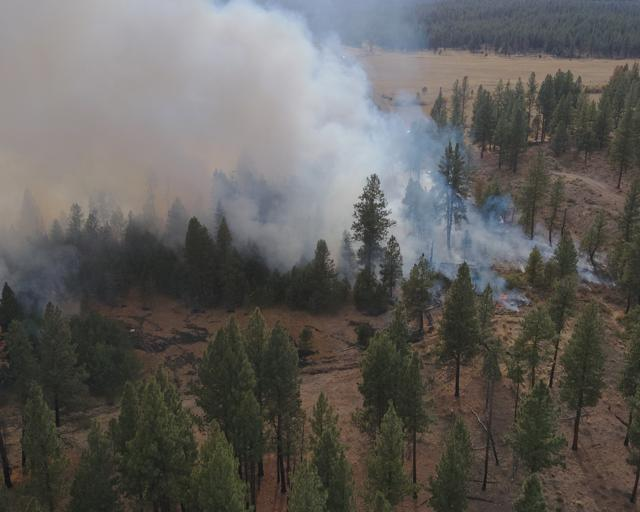
\includegraphics[width=0.47\textwidth]{./figures/sample_rgb.jpeg}}{\fbox{\parbox[c][4.5cm][c]{0.44\textwidth}{\centering\todo{figures/sample\_rgb.jpeg not found}}}}\hfill
  \IfFileExists{./figures/sample_thermal.jpeg}{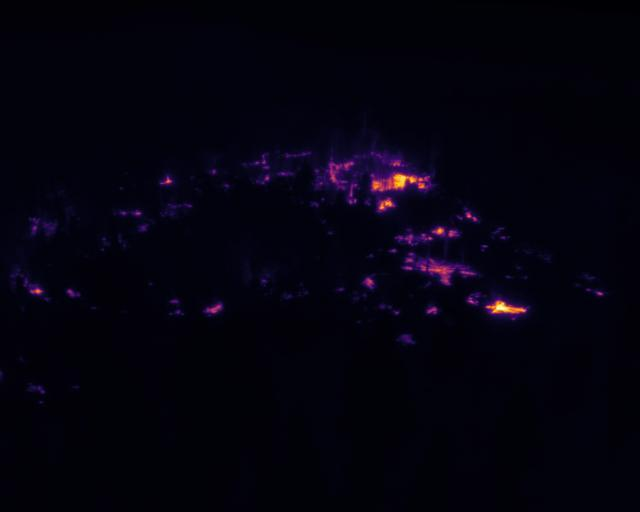
\includegraphics[width=0.47\textwidth]{./figures/sample_thermal.jpeg}}{\fbox{\parbox[c][4.5cm][c]{0.44\textwidth}{\centering\todo{figures/sample\_thermal.jpeg not found}}}}\\[4pt]
  \small(a) Visible image \hspace{0.32\textwidth} (b) Thermal image
  \caption{Example test image pair from the Sycan Marsh subset.}
  \label{fig:sample}
\end{figure}

\subsection{Experiment Configurations}
 Table~\ref{tab:variants} and Fig.~\ref{fig:placement} summarize the experimental configurations. Every configuration was implemented and trained on both the Qwen2-1.5B and Llama-3.2-1B backbones across all 16 fine-tuning runs. Low-rank adapters are applied either to attention projections (query $q$, key $k$, value $v$, output $o$) or to all linear projections across attention and feedforward MLP blocks (including gate, up, and down projections). The adapter design prioritizes parameter efficiency: the aim is to attain strong task accuracy with minimal parameter additions. Time limitations and preliminary observations from earlier experiments informed the distribution of rank sweeps across configurations. Across all fine-tuned models, the vision encoder remains frozen while the two projectors and modality embeddings are trained.

\begin{figure}[htbp]
  \centering
  \resizebox{\textwidth}{!}{%
  \begin{tikzpicture}[x=1.25cm, y=0.9cm, every node/.style={font=\footnotesize},
      mod/.style={draw, minimum width=1.1cm, minimum height=0.65cm, rounded corners=1pt},
      on/.style={mod, fill=orange!35}]
    \foreach \m [count=\i] in {q,k,v,o,gate,up,down}{
      \foreach \r in {0,-1,-2}{ \node[mod] at (\i,\r) {\m}; } }
    % adapted modules
    \foreach \i/\m in {1/q,3/v}{ \node[on] at (\i,0) {\m}; }
    \foreach \i/\m in {1/q,2/k,3/v,4/o}{ \node[on] at (\i,-1) {\m}; }
    \foreach \i/\m in {1/q,2/k,3/v,4/o,5/gate,6/up,7/down}{ \node[on] at (\i,-2) {\m}; }
    \node[anchor=east] at (0.35,0) {$q,v$};
    \node[anchor=east] at (0.35,-1) {$q,k,v,o$};
    \node[anchor=east] at (0.35,-2) {all-linear};
    \node[anchor=west] at (7.65,0) {$r\in\{8,16\}$};
    \node[anchor=west] at (7.65,-1) {$r\in\{4,8,16,32\}$};
    \node[anchor=west] at (7.65,-2) {$r\in\{8,16\}$};
    \draw[decorate, decoration={brace, amplitude=4pt}] (0.6,0.55) -- (4.4,0.55) node[midway, above=4pt] {self-attention};
    \draw[decorate, decoration={brace, amplitude=4pt}] (4.6,0.55) -- (7.4,0.55) node[midway, above=4pt] {MLP};
  \end{tikzpicture}}
  \caption{Linear modules of a decoder layer that receive LoRA adapters (shaded) in each configuration, and the ranks tested for it, for both backbones.}
  \label{fig:placement}
\end{figure}

\begin{table}[htbp]
  \centering
  \caption{The experimental configurations evaluated in this study (each configuration was trained on both Qwen2-1.5B and Llama-3.2-1B backbones)}
  \label{tab:variants}
  \begin{tabular}{P{1.8in}P{1.6in}cc}
    \toprule
    \textbf{Variant} & \textbf{Adapted modules} & \textbf{Rank $r$} & \textbf{$\alpha$} \\
    \midrule
    Frozen baseline (Qwen2.5-VL-3B) & none & --- & --- \\
    LoRA efficient & $q,v$ & 8, 16 & $2r$ \\
    LoRA balanced & $q,k,v,o$ & 4, 8, 16, 32 & $2r$ \\
    LoRA high capacity & all linear ($q,k,v,o$, gate, up, down) & 8, 16 & $2r$ \\
    \bottomrule
  \end{tabular}
\end{table}

\subsection{Hyperparameters}
Table~\ref{tab:hparams} presents the hyperparameter configurations across all 16 fine-tuning runs for both Qwen2-1.5B and Llama-3.2-1B backbones.
\begin{table}[htbp]
  \centering
  \caption{Training hyperparameters across all Qwen2-1.5B and Llama-3.2-1B fine-tuning runs}
  \label{tab:hparams}
  \footnotesize
  \setlength{\tabcolsep}{2.5pt}
  \resizebox{\textwidth}{!}{%
  \begin{tabular}{llcccccccccc}
    \toprule
    \textbf{Backbone} & \textbf{Adapters, rank} & \textbf{Optimizer} & \textbf{LR} & \textbf{Scheduler} & \textbf{Epochs (plan)} & \textbf{Epochs (done)} & \textbf{BS} & \textbf{GA} & \textbf{Eff.\ BS} & \textbf{Patience} & \textbf{Min $\Delta$} \\
    \midrule
    Qwen2-1.5B & $q,v$, $r{=}8$ & AdamW & 2e-4 & cosine+warmup & 100 & 12 & 4 & 4 & 16 & 3 & 1e-8 \\
    Qwen2-1.5B & $q,v$, $r{=}16$ & AdamW & 2e-4 & cosine+warmup & 100 & 12 & 4 & 4 & 16 & 3 & 1e-8 \\
    Qwen2-1.5B & $q,k,v,o$, $r{=}4$ & AdamW & 2e-4 & cosine+warmup & 100 & 14 & 4 & 4 & 16 & 3 & 1e-8 \\
    Qwen2-1.5B & $q,k,v,o$, $r{=}8$ & AdamW & 2e-4 & cosine+warmup & 100 & 13 & 4 & 4 & 16 & 3 & 1e-8 \\
    Qwen2-1.5B & $q,k,v,o$, $r{=}16$ & AdamW & 2e-4 & cosine+warmup & 100 & 10 & 4 & 4 & 16 & 3 & 1e-8 \\
    Qwen2-1.5B & $q,k,v,o$, $r{=}32$ & AdamW & 2e-4 & cosine+warmup & 100 & 13 & 4 & 4 & 16 & 3 & 1e-8 \\
    Qwen2-1.5B & all-linear, $r{=}8$ & AdamW & 2e-4 & cosine+warmup & 100 & 15 & 4 & 4 & 16 & 3 & 1e-8 \\
    Qwen2-1.5B & all-linear, $r{=}16$ & AdamW & 2e-4 & cosine+warmup & 100 & 13 & 4 & 4 & 16 & 3 & 1e-8 \\
    \midrule
    Llama-3.2-1B & $q,v$, $r{=}8$ & AdamW & 2e-4 & cosine+warmup & 100 & 10 & 4 & 4 & 16 & 3 & 1e-3 \\
    Llama-3.2-1B & $q,v$, $r{=}16$ & AdamW & 1.5e-4 & cosine+warmup & 10 & 7 & 4 & 4 & 16 & 3 & 1e-3 \\
    Llama-3.2-1B & $q,k,v,o$, $r{=}4$ & AdamW & 1.5e-4 & cosine+warmup & 10 & 8 & 4 & 4 & 16 & 3 & 1e-3 \\
    Llama-3.2-1B & $q,k,v,o$, $r{=}8$ & AdamW & 1.5e-4 & cosine+warmup & 10 & 9 & 4 & 4 & 16 & 3 & 1e-3 \\
    Llama-3.2-1B & $q,k,v,o$, $r{=}16$ & AdamW & 1.5e-4 & cosine+warmup & 8 & 8 & 4 & 4 & 16 & 2 & 1e-3 \\
    Llama-3.2-1B & $q,k,v,o$, $r{=}32$ & AdamW & 1.5e-4 & cosine+warmup & 10 & 8 & 4 & 4 & 16 & 3 & 1e-3 \\
    Llama-3.2-1B & all-linear, $r{=}8$ & AdamW & 1.5e-4 & cosine+warmup & 10 & 9 & 4 & 4 & 16 & 3 & 1e-3 \\
    Llama-3.2-1B & all-linear, $r{=}16$ & AdamW & 1e-4 & cosine+warmup & 100 & 9 & 2 & 8 & 16 & 3 & 1e-3 \\
    \bottomrule
  \end{tabular}}\\[2pt]
  {\footnotesize BS: per-device batch size; GA: gradient accumulation steps; Eff.\ BS: effective batch size (BS $\times$ GA = 16 across all runs); Min $\Delta$: early-stopping minimum improvement delta. Weight decay is 0.01, LoRA dropout is 0.05, LoRA $\alpha = 2r$, and warmup ratio is 0.05 for all 16 runs.}
\end{table}

Both backbones share the same random seed (42) and identical pairing audit files. All runs maintain an effective batch size of 16 (batch size 4 with 4 gradient accumulation steps, except the Llama all-linear $r{=}16$ run which used batch size 2 with 8 accumulation steps). The Qwen2 fine-tuning runs plan for 100 epochs (totaling 125,800 gradient steps with a 5\% warmup of 6,290 steps, or 5 epochs); because early stopping with $\text{MIN\_DELTA} = 10^{-8}$ halts training within 10 to 15 epochs, the learning rate ramps over the initial 5 epochs and remains above 95\% of its peak throughout the rest of training. In contrast, Llama runs are planned for 8 to 10 epochs (except all-linear $r{=}16$ planned for 100 epochs, and $q,v$ $r{=}8$ with learning rate $2\times 10^{-4}$) and use early-stopping threshold $\text{MIN\_DELTA} = 10^{-3}$, decaying fully over their horizon. The frozen in-context baseline utilizes 4-bit NF4 quantization, sets \texttt{min\_pixels} and \texttt{max\_pixels} to $224 \times 224$ in the image processor, greedy single-beam decoding, and a 32-token generation cap.

\subsection{Trainable Parameter Count}
For a linear layer with input dimension $d_{\text{in}}$ and output dimension $d_{\text{out}}$, rank-$r$ adaptation introduces $r(d_{\text{in}} + d_{\text{out}})$ trainable weights. In Qwen2-1.5B (28 Transformer layers, hidden dimension $d=1536$, 2 key/value heads of dimension 128 yielding $d_{\text{kv}}=256$, and MLP intermediate dimension 8960), each layer adds:
\begin{itemize}[leftmargin=0.5in, itemsep=1pt]
  \item $q$ projection: $r(1536 + 1536) = r(3072)$ parameters,
  \item $k$ and $v$ projections: $r(1536 + 256) = r(1792)$ parameters each,
  \item $o$ projection: $r(1536 + 1536) = r(3072)$ parameters,
  \item gate, up, and down projections: $r(1536 + 8960) = r(10496)$ parameters each.
\end{itemize}
The dual two-layer MLP projectors map the 768-dimensional visual tokens to dimension 1024 and then to language-model dimension 1536 ($768 \to 1024 \to 1536$), with learned bias vectors on each linear transformation. Each projector comprises:
\begin{align}
\text{Layer 1 weights and biases:} \quad & 768 \times 1024 + 1024 = 786{,}432 + 1{,}024 = 787{,}456, \\
\text{Layer 2 weights and biases:} \quad & 1024 \times 1536 + 1536 = 1{,}572{,}864 + 1{,}536 = 1{,}574{,}400, \\
\text{Single projector subtotal:} \quad & 787{,}456 + 1{,}574{,}400 = 2{,}361{,}856.
\end{align}
Across the two independent projectors (visible and thermal), this yields $2 \times 2{,}361{,}856 = 4{,}723{,}712$ parameters. The learned 1D modality type embeddings (\texttt{rgb\_type} and \texttt{thermal\_type}) each have dimension $1 \times 1 \times 1536$, contributing $2 \times 1536 = 3{,}072$ parameters. The complete non-adapter trainable parameter overhead is therefore:
\begin{equation}
4{,}723{,}712 + 3{,}072 = 4{,}726{,}784 \text{ parameters}.
\end{equation}
Table~\ref{tab:params} details the breakdown between adapter weights, projection weights, and total trainable parameters across all Qwen2-1.5B variants.
\begin{table}[htbp]
  \centering
  \caption{Trainable parameters of the Qwen2-1.5B variants}
  \label{tab:params}
  \small
  \begin{tabular}{@{}l>{\centering\arraybackslash}p{1.3in}>{\centering\arraybackslash}p{1.7in}>{\centering\arraybackslash}p{1.2in}@{}}
    \toprule
    \textbf{Variant} & \textbf{LoRA parameters} & \textbf{Projectors + modality embeddings} & \textbf{Total trainable} \\
    \midrule
    $q,k,v,o$, $r{=}4$ & 1,089,536 & 4,726,784 & 5,816,320 \\
    $q,v$, $r{=}8$ & 1,089,536 & 4,726,784 & 5,816,320 \\
    $q,k,v,o$, $r{=}8$ & 2,179,072 & 4,726,784 & 6,905,856 \\
    $q,v$, $r{=}16$ & 2,179,072 & 4,726,784 & 6,905,856 \\
    $q,k,v,o$, $r{=}16$ & 4,358,144 & 4,726,784 & 9,084,928 \\
    $q,k,v,o$, $r{=}32$ & 8,716,288 & 4,726,784 & 13,443,072 \\
    all-linear, $r{=}8$ & 9,232,384 & 4,726,784 & 13,959,168 \\
    all-linear, $r{=}16$ & 18,464,768 & 4,726,784 & 23,191,552 \\
    \bottomrule
  \end{tabular}\\[2pt]
  {\footnotesize Projectors ($768\to 1024\to 1536$) and modality type embeddings contribute $2 \times (768\times 1024 + 1024 + 1024\times 1536 + 1536) + 2 \times 1536 = 4,726,784$ parameters across all runs. LoRA parameter counts are derived from $r(d_{\text{in}} + d_{\text{out}})$ per target matrix across 28 layers.}
\end{table}


For Llama-3.2-1B (16 Transformer layers, hidden dimension $d=2048$, 8 query heads, 2 key/value heads with head dimension 128 yielding $d_{\text{kv}}=512$, and intermediate MLP dimension 8192), each layer adds:
\begin{itemize}[leftmargin=0.5in, itemsep=1pt]
  \item $q$ projection: $r(2048 + 2048) = r(4096)$ parameters,
  \item $k$ and $v$ projections: $r(2048 + 512) = r(2560)$ parameters each,
  \item $o$ projection: $r(2048 + 2048) = r(4096)$ parameters,
  \item gate, up, and down projections: $r(2048 + 8192) = r(10240)$ parameters each.
\end{itemize}
The dual two-layer MLP projectors map the 768-dimensional visual tokens to dimension 1024 and then to language-model dimension 2048 ($768 \to 1024 \to 2048$), with learned bias vectors on each linear transformation. Each projector comprises:
\begin{align}
\text{Layer 1 weights and biases:} \quad & 768 \times 1024 + 1024 = 786{,}432 + 1{,}024 = 787{,}456, \\
\text{Layer 2 weights and biases:} \quad & 1024 \times 2048 + 2048 = 2{,}097{,}152 + 2{,}048 = 2{,}099{,}200, \\
\text{Single projector subtotal:} \quad & 787{,}456 + 2{,}099{,}200 = 2{,}886{,}656.
\end{align}
Across both projectors, this contributes $2 \times 2{,}886{,}656 = 5{,}773{,}312$ parameters. The learned 1D modality type embeddings (\texttt{rgb\_type} and \texttt{thermal\_type}) each have dimension $1 \times 1 \times 2048$, contributing $2 \times 2048 = 4{,}096$ parameters. The non-adapter trainable parameter overhead for Llama-3.2-1B is therefore:
\begin{equation}
5{,}773{,}312 + 4{,}096 = 5{,}777{,}408 \text{ parameters}.
\end{equation}
Table~\ref{tab:llama_params} details the trainable parameter breakdown across all Llama-3.2-1B variants.
\begin{table}[htbp]
  \centering
  \caption{Trainable parameters of the Llama-3.2-1B variants}
  \label{tab:llama_params}
  \small
  \begin{tabular}{@{}l>{\centering\arraybackslash}p{1.3in}>{\centering\arraybackslash}p{1.7in}>{\centering\arraybackslash}p{1.2in}@{}}
    \toprule
    \textbf{Variant} & \textbf{LoRA parameters} & \textbf{Projectors + modality embeddings} & \textbf{Total trainable} \\
    \midrule
    $q,k,v,o$, $r{=}4$ & 851,968 & 5,777,408 & 6,629,376 \\
    $q,v$, $r{=}8$ & 851,968 & 5,777,408 & 6,629,376 \\
    $q,k,v,o$, $r{=}8$ & 1,703,936 & 5,777,408 & 7,481,344 \\
    $q,v$, $r{=}16$ & 1,703,936 & 5,777,408 & 7,481,344 \\
    $q,k,v,o$, $r{=}16$ & 3,407,872 & 5,777,408 & 9,185,280 \\
    all-linear, $r{=}8$ & 5,636,096 & 5,777,408 & 11,413,504 \\
    $q,k,v,o$, $r{=}32$ & 6,815,744 & 5,777,408 & 12,593,152 \\
    all-linear, $r{=}16$ & 11,272,192 & 5,777,408 & 17,049,600 \\  % CHECK: old table said 19,271,680 params for this run; formula gives this value
    \bottomrule
  \end{tabular}\\[2pt]
  {\footnotesize Projectors ($768\to 1024\to 2048$) and modality type embeddings contribute $2 \times (768\times 1024 + 1024 + 1024\times 2048 + 2048) + 2 \times 2048 = 5,777,408$ parameters across all runs. LoRA parameter counts are derived from $r(d_{\text{in}} + d_{\text{out}})$ per target matrix across 16 layers.}
\end{table}

% src: D-01, D-02, DS-005, DS-006, DS-007, DS-008, DS-009, DS-011, DS-012, DS-013, DS-014, DS-016, DS-018, DS-019, DS-020, DS-022, DS-023, DS-024, DS-025, DS-026, DS-036, DS-037, DS-039, balanced_qkvo_r16-001, balanced_qkvo_r16-002, balanced_qkvo_r16-003, balanced_qkvo_r16-004, balanced_qkvo_r16-005, balanced_qkvo_r16-006, balanced_qkvo_r16-007, balanced_qkvo_r16-015, balanced_qkvo_r16-016, balanced_qkvo_r16-017, balanced_qkvo_r16-018, balanced_qkvo_r16-019, balanced_qkvo_r16-020, balanced_qkvo_r16-021, balanced_qkvo_r16-022, balanced_qkvo_r16-023, balanced_qkvo_r16-047, balanced_qkvo_r4-029, efficient_qv_r8-023, qwen2_1_5b_balanced_qkvo_r16-001, qwen2_1_5b_balanced_qkvo_r16-010, qwen2_1_5b_balanced_qkvo_r16-014, qwen2_1_5b_balanced_qkvo_r16-021
% ---------------- CHAPTER 5 ------------------------------------------
\clearpage
\chapter{System Implementation}
\section{Modular Architecture}
The system implementation decomposes into six discrete components:
\begin{itemize}[leftmargin=0.5in, itemsep=2pt]
  \item \textbf{Data Ingestion and Pairing Module}: Downloads the WildFireVQA annotations and FLAME~3 imagery, executes the radiometric temperature signature verification across 738 image pairs, eliminates duplicate query records, and establishes the image-grouped 80/10/10 partitions.
  \item \textbf{Vision Encoding and Caching Module}: Pre-extracts 49 patch visual tokens ($7\times7$ grid) from each unique image using the frozen CLIP ViT-B/32 encoder and stores embeddings in memory, eliminating redundant vision forward passes during training iterations.
  \item \textbf{Prompt and Modality Projection Module}: Projects the 768-dimensional visible and thermal visual tokens through dedicated two-layer MLP projectors to the language model dimension, appends learned 1D modality type embeddings, and formats the multimodal token sequence alongside the query according to the target chat template.
  \item \textbf{Model Loading and Quantization Module}: Initializes the decoder language model (Qwen2-1.5B or Llama-3.2-1B) under 4-bit NormalFloat (NF4) quantization with double quantization and FP16 compute precision, attaches trainable LoRA matrices to designated linear projections, and sets non-adapted base parameters to frozen mode.
  \item \textbf{Supervised Training Module}: Trains adapter and projector parameters using cross-entropy loss computed strictly over target answer tokens, using the AdamW optimizer with cosine learning rate scheduling, warmup, and validation loss early stopping.
  \item \textbf{Inference and Evaluation Module}: Executes deterministic greedy decoding (one beam, maximum 32 generated tokens) and computes exact match, smoothed sentence BLEU-4, and ROUGE-L metrics against reference answers.
\end{itemize}

\section{Implementation Details}
Experiments are implemented across modular standalone environments corresponding to each configuration:
\begin{itemize}[leftmargin=0.5in, itemsep=2pt]
  \item Frozen few-shot baseline: \texttt{firevlm-few-shot-qwen-pre-trained}
  \item Qwen2-1.5B fine-tuning: \texttt{firevlm-qwen2-vl-1.5b-lora-*} covering $q,v$ ($r\in\{8, 16\}$), $q,k,v,o$ ($r\in\{4, 8, 16, 32\}$), and all-linear ($r\in\{8, 16\}$)
  \item Llama-3.2-1B fine-tuning: \texttt{firevlm-lora-*} covering $q,v$ ($r\in\{8, 16\}$), $q,k,v,o$ ($r\in\{4, 8, 16, 32\}$), and all-linear ($r\in\{8, 16\}$)
\end{itemize}
An early trial script with subsampled data ($N=3000$) served as a preliminary pipeline test and is not part of the evaluated experimental runs.

\subsection{Frozen Pretrained Baseline}
The few-shot baseline evaluates Qwen2.5-VL-3B-Instruct in 4-bit precision with all parameters frozen ($trainable = 0$). Test queries consist of 200 question--answer rows sampled from held-out images. For each query, a deterministic ordered pool of 10 demonstration examples from the same question category is constructed. The $k$-shot evaluation evaluates the first $k$ demonstration pairs ($k \in \{0, 1, \dots, 10\}$), providing strictly paired incremental context. Prompts include the visible and thermal images of each demonstration and query, formatted with system instructions to return concise answers. Confidence intervals are estimated using 1,000 bootstrap resamples.

\subsection{QLoRA Parameter-Efficient Fine-Tuning}
For the Qwen2 fine-tuning runs, the model is initialized from the \texttt{mit-han-lab/\allowbreak Qwen2-VL-1.5B-Instruct} repository \cite{mithan}.
The base weights are quantized to 4-bit NF4 representation and frozen. Only the low-rank adapter matrices, the dual modality projectors, and the two modality type embeddings require gradient updates. Training executes with effective batch size 16 (batch size 4, gradient accumulation steps 4; batch size 2 and accumulation 8 for Llama all-linear $r{=}16$). Validation loss is evaluated at the conclusion of each epoch, and the checkpoint achieving minimum validation loss is preserved for final evaluation on the 2,482 test rows. Fig.~\ref{fig:trainflow} summarises this procedure.

\begin{figure}[htbp]
  \centering
  \resizebox{\textwidth}{!}{%
  \begin{tikzpicture}[node distance=5mm and 7mm]
    \node[blk] (m) {Train manifest\\(20,128 rows)};
    \node[blk, right=of m] (f) {Cached CLIP\\tokens};
    \node[blk, right=of f] (t) {Forward pass,\\loss on answer tokens};
    \node[blk, right=of t] (u) {AdamW update\\(adapters, projectors)};
    \node[blk, below=10mm of u] (v) {Validation loss\\(each epoch)};
    \node[blk, left=of v, text width=30mm] (es) {Early stopping\\(patience 2 or 3)};
    \node[blk, left=of es, fill=green!12] (ck) {Keep best\\checkpoint};
    \node[blk, left=of ck] (ts) {Evaluate on\\2,482 test rows};
    \draw[arr] (m)--(f); \draw[arr] (f)--(t); \draw[arr] (t)--(u); \draw[arr] (u)--(v);
    \draw[arr] (v)--(es); \draw[arr] (es)--(ck); \draw[arr] (ck)--(ts);
  \end{tikzpicture}}
  \caption{Training and checkpoint-selection procedure used for every fine-tuning run. The checkpoint with the lowest validation loss is the one evaluated.}
  \label{fig:trainflow}
\end{figure}

\subsection{Answer Generation and Evaluation Protocol}
Answer generation operates deterministically via greedy decoding (do\_sample = False, num\_beams = 1) up to 32 new tokens. Only the initial text line prior to any newline character is extracted. A prediction is scored as an exact match (EM = 1) if it strictly matches the reference string following lowercasing and leading/trailing whitespace removal; otherwise EM = 0. The evaluation also computes smoothed sentence BLEU-4 and ROUGE-L. Normalized exact match (which additionally strips articles and punctuation) is tracked in the baseline. Because the reference answers consist predominantly of concise one- or two-word phrases, exact match serves as the primary metric. Fig.~\ref{fig:emflow} shows the post-processing and scoring chain.

\begin{figure}[htbp]
  \centering
  \resizebox{\textwidth}{!}{%
  \begin{tikzpicture}[node distance=6mm]
    \node[blk] (g) {Greedy decoding\\(max.\ 32 tokens)};
    \node[blk, right=of g] (l) {Keep first line\\of output};
    \node[blk, right=of l] (n) {Lower-case,\\trim whitespace};
    \node[blk, right=of n] (c) {String equality\\with reference};
    \node[blk, right=of c, fill=green!12] (e) {EM $=1$ or $0$};
    \draw[arr] (g)--(l); \draw[arr] (l)--(n); \draw[arr] (n)--(c); \draw[arr] (c)--(e);
  \end{tikzpicture}}
  \caption{Answer post-processing and exact-match scoring.}
  \label{fig:emflow}
\end{figure}
% src: D-06, D-08, DS-004, DS-011, DS-027, DS-030, DS-031, DS-032, DS-033, DS-035, DS-038, FS-001, FS-004, FS-005, FS-006, FS-007, FS-009, FS-010, FS-011, FS-012, FS-013, FS-014, FS-015, FS-016, FS-056, FS-057, FS-059, FS-071, FS-072, balanced_qkvo_r16-008, balanced_qkvo_r16-010, balanced_qkvo_r16-011, balanced_qkvo_r16-012, balanced_qkvo_r16-016, balanced_qkvo_r16-017, balanced_qkvo_r16-018, balanced_qkvo_r16-019, balanced_qkvo_r16-020, balanced_qkvo_r16-023, balanced_qkvo_r16-024, balanced_qkvo_r16-025, balanced_qkvo_r16-026, balanced_qkvo_r16-047, balanced_qkvo_r16-048, balanced_qkvo_r16-049, balanced_qkvo_r4-029, qwen2_1_5b_balanced_qkvo_r16-010

% ---------------- CHAPTER 6 ------------------------------------------
\clearpage
\chapter{System Testing}
\section{Testing Approach}
The system is an offline experimental pipeline rather than an interactive application, so testing concentrates on three questions: whether the data fed to every run is correct and leak-free, whether each model trains only the parameters it is meant to train, and whether each complete run produces a full, internally consistent set of predictions. Checks are written as \texttt{assert} statements inside the notebooks, so a violated condition stops the run before any result is produced; they were therefore executed on every run of the corresponding notebook. Four levels were used (Fig.~\ref{fig:testlevels}), and Table~\ref{tab:testcases} lists the 14 test cases with their expected and observed results.
\begin{itemize}[leftmargin=0.5in, itemsep=2pt]
  \item \textbf{Data validation tests} (TC-01 to TC-06): pairing, duplicates, split sizes, split disjointness and modality divergence.
  \item \textbf{Model and training tests} (TC-07 to TC-10): frozen baseline, adapter scoping, trainable-parameter scope and GPU placement.
  \item \textbf{System tests} (TC-11 to TC-14): end-to-end completion, metric consistency, reproducibility of inputs and baseline completion.
  \item \textbf{Non-functional checks}: whether every run fits the single T4 GPU, plus the training time and baseline latency that were logged.
\end{itemize}

\begin{figure}[htbp]
  \centering
  \resizebox{\textwidth}{!}{%
  \begin{tikzpicture}[node distance=5mm and 6mm,
      gate/.style={draw, dashed, rounded corners=2pt, fill=orange!12, font=\footnotesize, align=center, inner sep=2pt}]
    % row 1: data stages
    \node[blk] (a) {Raw\\annotations};
    \node[blk, right=of a] (b) {Pairing\\audit};
    \node[blk, right=of b] (c) {Deduplication};
    \node[blk, right=of c] (d) {Image-grouped\\split};
    \node[blk, right=of d] (e) {CLIP feature\\cache};
    % row 2: model stages
    \node[blk, below=14mm of e] (f) {Quantized LLM\\+ LoRA};
    \node[blk, left=of f] (g) {Training\\(early stopping)};
    \node[blk, left=of g] (h) {Test\\generation};
    \node[blk, left=of h] (i) {Scoring\\(EM, ROUGE-L)};
    \draw[arr] (a)--(b); \draw[arr] (b)--(c); \draw[arr] (c)--(d); \draw[arr] (d)--(e);
    \draw[arr] (e)--(f); \draw[arr] (f)--(g); \draw[arr] (g)--(h); \draw[arr] (h)--(i);
    % gates
    \node[gate, above=4mm of b] {TC-01, TC-02\\pairing, 34 per pair};
    \node[gate, above=4mm of c] {TC-03\\no duplicates};
    \node[gate, above=4mm of d] {TC-04, TC-05\\disjoint, sizes};
    \node[gate, above=4mm of e] {TC-06\\RGB $\ne$ thermal};
    \node[gate, below=4mm of f] {TC-08 to TC-10\\adapters, scope, GPU};
    \node[gate, below=4mm of h] {TC-11, TC-12\\2,482 rows, counts};
    \node[gate, below=4mm of i] {TC-13\\same inputs};
  \end{tikzpicture}}
  \caption{Test levels and where each check sits in the pipeline. Dashed boxes are the checks of Table~\ref{tab:testcases}.}
  \label{fig:testlevels}
\end{figure}

\section{Test Environment}
All tests ran on the Kaggle Tesla T4 environment of Chapter~3 (single GPU, 14.6\,GiB, PyTorch 2.11.0, \texttt{transformers} 4.57.1, \texttt{peft} 0.17.1). No separate test machine or test framework was used: the checks live in the same notebooks that train and evaluate the models.

\section{Data Validation Tests}
\textbf{TC-01 to TC-03: pairing and duplicates.} The pairing audit asserted a one-to-one mapping between source image keys and canonical target stems, and an assertion after deduplication verified that no image carries a repeated question (all 16 fine-tuning notebooks).
\begin{lstlisting}
assert len(source_to_target) == len(source_meta)
assert len(set((row.source_class, source_to_target[row.source_image_key]) for row in source_meta.itertuples())) == len(source_meta)
assert not duplicate_questions.any()
\end{lstlisting}
The printed output confirms that all 738 source image pairs were matched (734 exact and 4 tolerance matches) with 34 questions per pair.

\textbf{TC-04 and TC-05: split disjointness and sizes.} The train (592 images), validation (73) and test (73) partitions were asserted to be mutually disjoint for both visible and thermal paths. Row counts follow from the 34 questions per image: $592\times34=20{,}128$, $73\times34=2{,}482$, and $20{,}128+2{,}482+2{,}482=25{,}092$, the size of the Sycan Marsh subset.
\begin{lstlisting}
assert train_paths.isdisjoint(val_paths)
assert train_paths.isdisjoint(test_paths)
assert val_paths.isdisjoint(test_paths)
assert train_thermal.isdisjoint(val_thermal)
assert train_thermal.isdisjoint(test_thermal)
assert val_thermal.isdisjoint(test_thermal)
\end{lstlisting}

\textbf{TC-06: modality divergence.} To catch a path-resolution error that would feed the same image to both encoders, the extracted CLIP features of the visible and thermal images were required to differ.
\begin{lstlisting}
assert _diff > 1e-4, 'RGB and thermal features look identical; check path resolution.'
\end{lstlisting}

\section{Model and Training Tests}
\textbf{TC-07: frozen baseline.} The few-shot baseline asserted that no parameter requires a gradient and that demonstration images never coincide with query images.
\begin{lstlisting}
trainable = sum(p.numel() for p in model.parameters() if p.requires_grad)
assert trainable == 0, 'Few-shot baseline must not update model weights.'
assert set(support_df['rgb_resolved']).isdisjoint(set(test_df['rgb_resolved']))
assert set(support_df['thermal_resolved']).isdisjoint(set(test_df['thermal_resolved']))
\end{lstlisting}

\textbf{TC-08 to TC-10: adapters, parameter scope and GPU.} In the seven Qwen2 notebooks with adapter inspection, the number of adapted layers had to equal the number of target modules times the number of decoder layers, with the configured rank. Printed outputs confirm that the trainable parameters are only the adapter matrices, the two projectors and the two modality type embeddings. All 16 fine-tuning notebooks also asserted single-GPU placement.
\begin{lstlisting}
assert len(adapter_layers) == len(CFG.LORA_TARGET_MODULES) * backbone_config.num_hidden_layers
assert all(name.endswith(adapter_suffixes) for name, _ in adapter_layers)
assert all(module.lora_A['default'].weight.shape[0] == CFG.LORA_R for _, module in adapter_layers)
assert used_cuda_devices == {'cuda:0'}
\end{lstlisting}

\section{System-Level Tests}
\textbf{TC-11 and TC-12: completion and metric consistency.} Each of the 16 result files reports 2,482 scored samples, equal to the test manifest. The category counts (584, 584, 292, 438, 292, 292) sum to 2,482, and for the four runs analysed in Table~\ref{tab:category} the per-category correct counts sum to the run totals (2,150, 2,088, 2,144 and 2,196), so the reported percentages can be reproduced from integer counts.

\textbf{TC-13: reproducibility of inputs.} The pairing audit file is byte-identical across all 16 runs and the train, validation and test manifests are byte-identical across the eight Qwen2 runs, with split seed 42. Differences between runs therefore come from the adapter configuration and training settings, not from different data.

\textbf{TC-14: baseline completion.} The frozen baseline completed all 11 demonstration counts ($k=0,\dots,10$) on 200 queries each, 2{,}200 generations in total, with zero weight updates.

\section{Non-Functional Checks}
\textbf{Memory.} All 16 training runs and the baseline completed on a single 14.6\,GiB T4 using 4-bit NF4 weights, cached CLIP features and an effective batch size of 16. Peak GPU memory was not logged in the available outputs, so only completion without an out-of-memory error is claimed.

\textbf{Time.} The logged cumulative training time per fine-tuning run ranges from 28.8 to 55.6 minutes (Fig.~\ref{fig:minutes}). The frozen baseline mean latency rises from 0.40\,s at $k=0$ to 2.23\,s at $k=10$ (Fig.~\ref{fig:cost}). Inference latency of the fine-tuned models was not recorded.

\needspace{12\baselineskip}
\section{Test Case Summary}
{\footnotesize
\setlength{\tabcolsep}{3pt}
\renewcommand{\arraystretch}{1.15}
\begin{longtable}{P{0.4in}P{1.4in}P{1.4in}P{1.5in}P{0.4in}}
\caption{System test cases, expected results and observed outcomes}\label{tab:testcases}\\
\toprule
\textbf{ID} & \textbf{Test} & \textbf{Expected} & \textbf{Observed} & \textbf{Result} \\
\midrule
\endfirsthead
\multicolumn{5}{l}{\textit{Table \thetable\ (continued)}}\\
\toprule
\textbf{ID} & \textbf{Test} & \textbf{Expected} & \textbf{Observed} & \textbf{Result} \\
\midrule
\endhead
\midrule \multicolumn{5}{r}{\textit{Continued on next page}}\\
\endfoot
\bottomrule
\endlastfoot
TC-01 & One-to-one source-to-target pairing (16 notebooks) & Every source image maps to one canonical pair & 738 pairs matched: 734 exact, 4 tolerance & Pass \\
TC-02 & Questions per image pair & 34 per pair & 34 per pair; $738\times34=25{,}092$ rows & Pass \\
TC-03 & Duplicate questions after deduplication & None within an image & None found & Pass \\
TC-04 & Split image disjointness, visible and thermal paths & No image in two splits & Train 592, val 73, test 73, no overlap & Pass \\
TC-05 & Split size consistency & Rows $=34\times$ images & $20{,}128+2{,}482+2{,}482=25{,}092$ & Pass \\
TC-06 & Visible and thermal features differ & Mean difference $>10^{-4}$ & Assertion passed in all 16 notebooks & Pass \\
TC-07 & Frozen baseline & 0 trainable parameters; support disjoint from query & Both assertions passed & Pass \\
TC-08 & Adapter count and rank (7 Qwen2 notebooks) & Targets $\times$ layers adapters, rank $=r$ & Assertions passed & Pass \\
TC-09 & Trainable-parameter scope & Adapters, projectors, type embeddings only & Confirmed by printed output & Pass \\
TC-10 & Single GPU placement & All on \texttt{cuda:0} & Assertion passed in all 16 notebooks & Pass \\
TC-11 & End-to-end completion & 2,482 scored rows per run & 2,482 in all 16 result files & Pass \\
TC-12 & Metric consistency & Category counts and correct counts add up & 2,482 rows; 2,150, 2,088, 2,144, 2,196 correct & Pass \\
TC-13 & Same inputs across runs & Identical audit file and manifests & Byte-identical (16 and 8 runs) & Pass \\
TC-14 & Baseline completion & 11 shot counts, 2,200 generations & Completed; 0 weight updates & Pass \\
\end{longtable}}

\section{Defects Found and Limitations of the Testing}
\textbf{Defects found.} The checks and the audit exposed two problems that were not repaired. First, the baseline notebook resolves image paths with a simpler mapping than the audited pipeline: it assigns the 25,092 annotation rows to only 480 distinct RGB files (about 52 rows per file) instead of 34 questions for each of 738 pairs, so some baseline questions may have been shown the wrong image (Section~\ref{sec:evalsetup}); the baseline was not rerun and is reported as indicative only. Second, the per-site row counts sum to 207,298 while the reader loaded 207,306 rows (Section~\ref{sec:dataset}); the cause was not established and the study uses only the Sycan Marsh subset, which is unaffected.

\textbf{Limitations.} The tests are assertions inside notebooks, not an automated test suite that can be rerun independently. No adversarial, out-of-distribution or other-site input was tested, predictions were not reviewed by a wildfire expert, and the assertions confirm data and parameter correctness but not answer correctness, which is measured separately in Chapter~7.
% src: DS-009, DS-011, DS-013, DS-014, DS-018, DS-019 to DS-027, FS-058, FS-059, FS-071, FS-072; metrics_table.csv (n_samples = 2482, minutes 28.77 to 55.58); tab_category.tex counts; 592x34=20,128; 73x34=2,482; 738x34=25,092
% ---------------- CHAPTER 7 ------------------------------------------
\clearpage 
\chapter{Results and Analysis}

\section{Evaluation Framework}
\label{sec:evalsetup}
\textbf{Fine-tuned runs.} All 16 fine-tuned runs were scored on the test split of 73 held-out image pairs, which contains 2,482 question--answer rows (all 16 result files report 2,482 samples). Each configuration was trained once; the split seed is 42 and no configuration was repeated with another seed.

\textbf{Metric.} Exact match (EM) is the primary metric, because the expected answers are drawn from a very limited set and BLEU and ROUGE are considered unsuitable for this task by the project owner. A prediction scores 1 if it equals the reference after lower-casing and trimming whitespace (Chapter~5). ROUGE-L is listed for completeness. BLEU is not tabulated: across the 16 runs it lies between 0.137 and 0.150 and was not used to rank runs.

\textbf{Frozen baseline.} The frozen Qwen2.5-VL-3B-Instruct baseline is evaluated on 200 queries for each $k=0,\dots,10$ (2,200 generations, no weight updates). It is kept in the project for comparison only. The baseline notebook resolves image paths with a simpler mapping than the audited fine-tuning pipeline. That mapping assigns the 25,092 annotation rows to only 480 distinct RGB files, about 52 rows per file, whereas the audited pipeline has 738 image pairs with 34 questions each. Some baseline question rows may therefore have been paired with a different image than the one they were written for. The 200 baseline queries do not record an image key, so this could not be checked after the fact, the cause was not established, and the baseline was not rerun. The baseline results are therefore reported as an indicative reference for frozen in-context prompting only. They are not paired with the fine-tuned test split, and no conclusion in this chapter depends on them being so.
% src: D-03, D-04, D-06, DS-020, DS-025, FS-056, FS-057, FS-058, FS-059; metrics_table.csv (n_samples = 2482 for 16 runs; BLEU min 0.1374, max 0.1497); 480 files / 25,092 rows from the reviewer-confirmed baseline audit (480 vs 738, 52 vs 34 rows per image); 25,092/480 = 52.3

\section{Main Comparative Results}
Table~\ref{tab:results} lists the frozen baseline at $k=10$ and seven fine-tuned configurations. The best frozen setting reaches 28.00\% EM with ROUGE-L 0.3760. The fine-tuned runs reach 84.13\% to 88.48\% EM, which is 56 to 60 points higher than the best baseline setting. Because the baseline uses a different model, a different test sample and possibly mismatched images (Section~\ref{sec:evalsetup}), the size of this gap is indicative and is not a controlled measurement of the effect of fine-tuning. The Qwen2-1.5B and Llama-3.2-1B runs also differ in several training settings (Section~\ref{sec:llama}), so Table~\ref{tab:results} should not be read as a ranking of the two backbones.
\begin{table}[htbp]
  \centering
  \caption{Representative configurations: frozen in-context baseline and fine-tuned runs}
  \label{tab:results}
  \small
  \setlength{\tabcolsep}{4pt}
  \begin{tabular}{P{2.3in}ccc}
    \toprule
    \textbf{Configuration} & \textbf{Trainable params} & \textbf{EM (\%)} & \textbf{ROUGE-L} \\
    \midrule
    Frozen baseline, $k{=}10$ (Qwen2.5-VL-3B; 200 queries) & 0 & 28.00 & 0.3760 \\
    \midrule
    LoRA $q,k,v,o$, $r{=}4$ (Qwen2-1.5B) & 5,816,320 & 86.62 & 0.8979 \\
    LoRA $q,v$, $r{=}8$ (Qwen2-1.5B) & 5,816,320 & 86.14 & 0.8932 \\
    LoRA $q,k,v,o$, $r{=}16$ (Qwen2-1.5B) & 9,084,928 & 84.13 & 0.8773 \\
    LoRA all-linear, $r{=}8$ (Qwen2-1.5B) & 13,959,168 & 84.85 & 0.8858 \\
    LoRA $q,k,v,o$, $r{=}8$ (Llama-3.2-1B) & 7,481,344 & 88.48 & 0.9121 \\
    LoRA $q,v$, $r{=}8$ (Llama-3.2-1B) & 6,629,376 & 86.38 & 0.8911 \\
    LoRA all-linear, $r{=}16$ (Llama-3.2-1B) & 17,049,600 & 85.46 & 0.8878 \\  % CHECK: old table said 19,271,680 params for this run; formula gives this value
    \bottomrule
  \end{tabular}\\[2pt]
  {\footnotesize The baseline row uses 200 queries sampled separately from the fine-tuning test split and is an indicative reference only (Section~\ref{sec:evalsetup}); the fine-tuned rows use all 2,482 test rows. The Qwen2 and Llama runs differ in several training settings (Table~\ref{tab:hparams}).}
\end{table}

% src: FS-030, FS-041, FS-059, D-03, D-04; tables/tab_main_results.tex generated by tools/recompute_ch7.py from metrics_table.csv; 88.48-28.00 = 60.48, 84.13-28.00 = 56.13

\section{In-Context Few-Shot Baseline}
\label{sec:fewshot}
Table~\ref{tab:shots} and Fig.~\ref{fig:shots} give the frozen baseline for each number of demonstrations $k$.
\begin{table}[htbp]
  \centering
  \caption{Frozen Qwen2.5-VL-3B-Instruct performance across demonstration counts $k$ (200 test queries; brackets indicate 95\% bootstrap confidence intervals)}
  \label{tab:shots}
  \small
  \setlength{\tabcolsep}{4pt}
  \resizebox{\textwidth}{!}{%
  \begin{tabular}{cccccc}
    \toprule
    \textbf{$k$} & \textbf{EM (\%) [95\% CI]} & \textbf{ROUGE-L} & \textbf{Words / answer} & \textbf{Latency (s)} & \textbf{Input tokens} \\
    \midrule
    0 & 15.00 [10.5, 20.0] & 0.2438 & 2.51 & 0.40 & 211 \\
    1 & 20.00 [15.0, 25.5] & 0.3113 & 1.73 & 0.51 & 381 \\
    2 & 23.50 [18.5, 29.5] & 0.3280 & 1.54 & 0.65 & 552 \\
    3 & 23.50 [18.0, 30.0] & 0.3290 & 1.54 & 0.80 & 723 \\
    4 & 24.50 [18.5, 30.5] & 0.3362 & 1.60 & 0.98 & 893 \\
    5 & 25.50 [19.5, 32.0] & 0.3421 & 1.66 & 1.14 & 1,064 \\
    6 & 26.00 [20.0, 32.0] & 0.3474 & 1.67 & 1.33 & 1,235 \\
    7 & 27.00 [21.5, 33.5] & 0.3585 & 1.66 & 1.54 & 1,405 \\
    8 & 26.00 [20.5, 32.5] & 0.3468 & 1.66 & 1.76 & 1,576 \\
    9 & 27.50 [21.5, 34.0] & 0.3668 & 1.64 & 1.99 & 1,747 \\
    10 & 28.00 [22.0, 34.0] & 0.3760 & 1.61 & 2.23 & 1,919 \\
    \bottomrule
  \end{tabular}}
\end{table}

\begin{figure}[htbp]
  \centering
  \begin{tikzpicture}
    \begin{axis}[width=0.85\textwidth, height=6.2cm, xlabel={Number of demonstrations $k$},
      ylabel={Score (\%)}, xmin=0, xmax=10, ymin=10, ymax=42, xtick={0,1,...,10},
      legend pos=south east, grid=major, grid style={gray!25}, every axis plot/.append style={thick}]
      \addplot[mark=*, color=blue!70!black] coordinates {(0,15)(1,20)(2,23.5)(3,23.5)(4,24.5)(5,25.5)(6,26)(7,27)(8,26)(9,27.5)(10,28)};
      \addlegendentry{Exact match}
      \addplot[mark=square*, color=red!70!black] coordinates {(0,24.38)(1,31.13)(2,32.80)(3,32.90)(4,33.62)(5,34.21)(6,34.74)(7,35.85)(8,34.68)(9,36.68)(10,37.60)};
      \addlegendentry{ROUGE-L $\times$ 100}
    \end{axis}
  \end{tikzpicture}
  \caption{Exact match and ROUGE-L of the frozen baseline against the number of demonstrations (200 queries).}
  \label{fig:shots}
\end{figure}

\begin{figure}[htbp]
  \centering
  \begin{tikzpicture}
    \begin{axis}[width=0.85\textwidth, height=6.2cm, xlabel={Number of demonstrations $k$},
      ylabel={Exact match (\%)}, xmin=-0.3, xmax=10.3, ymin=0, ymax=40, xtick={0,1,...,10},
      grid=major, grid style={gray!25}, every axis plot/.append style={thick}]
      \addplot[mark=*, color=blue!70!black, error bars/.cd, y dir=both, y explicit]
        plot coordinates {
          (0,15)   +- (0,4.5) (1,20)   +- (0,5.0)
          (2,23.5) +- (0,5.5) (3,23.5) +- (0,6.0)
          (4,24.5) +- (0,6.0) (5,25.5) +- (0,6.5)
          (6,26)   +- (0,6.0) (7,27)   +- (0,6.5)
          (8,26)   +- (0,6.5) (9,27.5) +- (0,6.5) (10,28) +- (0,6.0)};
    \end{axis}
  \end{tikzpicture}
  \caption{Frozen-baseline exact match with 95\% bootstrap intervals (symmetrised to the larger half-width of Table~\ref{tab:shots}). The overlap of neighbouring intervals shows that adjacent values of $k$ cannot be separated with 200 queries.}
  \label{fig:shotci}
\end{figure}

\begin{figure}[htbp]
  \centering
  \begin{tikzpicture}
    \begin{axis}[width=0.85\textwidth, height=6.2cm, xlabel={Number of demonstrations $k$},
      axis y line*=left, ylabel={Mean latency (s)}, xmin=0, xmax=10, ymin=0, ymax=2.6,
      xtick={0,1,...,10}, grid=major, grid style={gray!25}, every axis plot/.append style={thick}]
      \addplot[mark=*, color=blue!70!black] coordinates {(0,0.40)(1,0.51)(2,0.65)(3,0.80)(4,0.98)(5,1.14)(6,1.33)(7,1.54)(8,1.76)(9,1.99)(10,2.23)};
    \end{axis}
    \begin{axis}[width=0.85\textwidth, height=6.2cm, axis y line*=right, axis x line=none,
      ylabel={Mean input tokens}, xmin=0, xmax=10, ymin=0, ymax=3200,
      every axis plot/.append style={thick}]
      \addplot[mark=square*, color=red!70!black] coordinates {(0,211)(1,381)(2,552)(3,723)(4,893)(5,1064)(6,1235)(7,1405)(8,1576)(9,1747)(10,1919)};
    \end{axis}
  \end{tikzpicture}
  \caption{Cost of in-context prompting: mean latency (blue circles, left axis) and mean input tokens (red squares, right axis) against the number of demonstrations.}
  \label{fig:cost}
\end{figure}

Exact match rises from 15.00\% at $k=0$ to 28.00\% at $k=10$, and ROUGE-L from 0.2438 to 0.3760. Relative to the zero-shot answers on the same queries, the gain is $+5.0$ points at $k=1$, $+8.5$ at $k=2$ and $k=3$, $+10.5$ at $k=5$, $+11.0$ at $k=8$ and $+13.0$ at $k=10$ (95\% bootstrap interval 8.0 to 18.5 points at $k=10$; 29 queries improved and 3 became worse). Most of the gain is reached by $k=2$. The curve is not monotone ($k=3$ equals $k=2$; $k=8$ is 1.0 point below $k=7$), and each 95\% interval in Table~\ref{tab:shots} is about 10 to 12.5 points wide, so differences between neighbouring values of $k$ are not resolved by 200 queries (Fig.~\ref{fig:shotci}). 

The mean answer length falls from 2.51 words at $k=0$ to 1.73 at $k=1$ and 1.54 at $k=2$, and stays between 1.54 and 1.67 words for $k\ge 2$. This chapter does not test whether the change in length accounts for the change in EM. The cost grows with $k$ (Fig.~\ref{fig:cost}): mean latency rises from 0.40\,s to 2.23\,s and the mean input from 211 to 1,919 tokens. Table~\ref{tab:fsexamples} shows ten queries; for the hottest-temperature question the reference is $>$500\textdegree C, the zero-shot answer is 400 and the ten-shot answer is 100.
\begin{table}[htbp]
  \centering
  \caption{Frozen few-shot predictions for ten test queries (exact match marked $\checkmark$)}
  \label{tab:fsexamples}
  \small
  \begin{tabular}{P{2.0in}P{0.95in}P{1.0in}P{1.0in}}
    \toprule
    \textbf{Question (abridged)} & \textbf{Reference} & \textbf{$k{=}0$} & \textbf{$k{=}10$} \\
    \midrule
    Most intense hotspot location & Center & Upper right & Bottom-right \\
    Region of largest smoke plume & Center & Top-left & Left \\
    Fuel-bed continuity & Continuous & (full sentence) & Continuous $\checkmark$ \\
    Hottest temperature (\textdegree C) & $>$500 & 400 & 100 \\
    Safety risk of UAV position & Medium risk & High & High \\
    Scene share above 200\textdegree C & $<$5\% & 50\% & 0\% \\
    Region of largest smoke plume & Bottom-left & Top-left & Top-left \\
    Number of emergency vehicles & 0 & 0 $\checkmark$ & 0 $\checkmark$ \\
    Primary ground fuel type & Grass & Vegetation & Grass $\checkmark$ \\
    Buildings visible & Yes & No & No \\
    \bottomrule
  \end{tabular}
\end{table}
% src: FS-020 to FS-041 (EM, ROUGE-L), FS-042 to FS-051 (paired deltas; the 8.0-18.5 interval and the 29/3 counts are carried from the previous draft: confirm against shot_summary.csv), FS-052 to FS-055 (latency, tokens, words), FS-056, FS-057; tab:fsexamples is unchanged from the previous draft and could not be re-checked from the attached files

\section{Qwen2-1.5B: Adapter Placement and Rank}
\label{sec:qwen}
Table~\ref{tab:ablation} lists all eight Qwen2-1.5B runs. The rank sweeps are not equally dense: $q,k,v,o$ was run at four ranks and $q,v$ and all-linear at two each, owing to time limits, and the $q,v$ setup was not extended further because it had not shown good results in other experiments.
\begin{table}[htbp]
  \centering
  \caption{Qwen2-1.5B fine-tuning runs (2,482 test rows, single seed; rows sorted by EM)}
  \label{tab:ablation}
  \footnotesize
  \setlength{\tabcolsep}{4pt}
  \resizebox{\textwidth}{!}{%
  \begin{tabular}{lrcccc}
    \toprule
    \textbf{Adapters, rank} & \textbf{Trainable params} & \textbf{EM (\%)} & \textbf{ROUGE-L} & \textbf{Min.\ val.\ loss} & \textbf{Epochs run} \\
    \midrule
    $q,k,v,o$, $r{=}4$ & 5,816,320 & 86.62 & 0.8979 & 0.1236 & 14 \\
    $q,k,v,o$, $r{=}8$ & 6,905,856 & 86.30 & 0.8928 & 0.1159 & 13 \\
    $q,v$, $r{=}8$ & 5,816,320 & 86.14 & 0.8932 & 0.1209 & 12 \\
    $q,v$, $r{=}16$ & 6,905,856 & 86.06 & 0.8937 & 0.1177 & 12 \\
    all-linear, $r{=}16$ & 23,191,552 & 85.74 & 0.8919 & 0.1209 & 13 \\
    $q,k,v,o$, $r{=}32$ & 13,443,072 & 85.50 & 0.8869 & 0.1191 & 13 \\
    all-linear, $r{=}8$ & 13,959,168 & 84.85 & 0.8858 & 0.1257 & 15 \\
    $q,k,v,o$, $r{=}16$ & 9,084,928 & 84.13 & 0.8773 & 0.1270 & 10 \\
    \bottomrule
  \label{tab:ablation}
  \end{tabular}}\\[2pt]
\end{table}

All eight runs lie between 84.13\% and 86.62\%. The four runs $q,k,v,o$ at $r=4$ and $r=8$ and $q,v$ at $r=8$ and $r=16$ span 86.06\% to 86.62\%, 0.56 points. The paired image-level bootstrap in Table~\ref{tab:bootstrap} gives intervals that contain zero for the differences among them, for example $q,k,v,o$ $r=4$ against $r=8$ ($+0.32$ points, interval $-0.99$ to $+1.63$). The $q,v$ run at $r=8$ has exactly the same number of trainable parameters as the best run (5,816,320) and is 0.48 points below it. These differences are small relative to the resolution of a single seed and a 73-image test set, and the runs are not ranked here.

The four remaining runs ($q,k,v,o$ $r=32$, all-linear $r=16$ and $r=8$, and $q,k,v,o$ $r=16$) are about 0.9 to 2.5 points below the best run. Only for $q,k,v,o$ $r=16$ does the interval exclude zero ($+2.50$ points, interval $+1.14$ to $+3.97$); for all-linear $r=8$ the lower end is $-0.04$. Within the tested configurations, larger trainable counts did not give higher exact match: the three runs with the most trainable parameters (23.2, 14.0 and 13.4 million) score 85.74\%, 84.85\% and 85.50\%, below the four runs with 5.8 to 6.9 million. Of these 5.8 to 6.9 million parameters, 4.7 million are the projectors and modality embeddings in every run, which is 81\% of the total in the smallest configurations. Why the larger adapters score lower was not investigated.

Every run was stopped by early stopping after 10 to 15 epochs of a planned 100. The lowest validation loss (0.1159, $q,k,v,o$ $r=8$) does not belong to the run with the highest test EM ($q,k,v,o$ $r=4$, minimum validation loss 0.1236, the third highest of the eight). Validation loss was used only to select the checkpoint of each run. Fig.~\ref{fig:valloss} plots the minimum validation loss against test EM for all 16 runs.
% src: D-01, D-02; metrics_table.csv via tools/recompute_ch7.py (EM, ROUGE-L, params, min val loss, epochs run); differences 0.564, 0.483, 0.322, 2.498, 1.128, 1.773, 0.886 (recompute_ch7.py); intervals from tools/cluster_bootstrap.py (see tab_bootstrap; to be rerun with 73 clusters); projector share 4,726,784 / 5,816,320 = 81.3\%

\begin{table}[htbp]
  \centering
  \caption[Exploratory paired image-level bootstrap of exact-match differences]{Exploratory paired image-level bootstrap of exact-match differences (points; 95\% percentile interval).}
  \label{tab:bootstrap}
  \footnotesize
  \setlength{\tabcolsep}{4pt}
  \begin{tabular}{P{3.1in}cc}
    \toprule
    \textbf{Comparison (A $-$ B)} & \textbf{$\Delta$ EM} & \textbf{95\% interval} \\
    \midrule
    Qwen2 $q,k,v,o$ $r{=}4$ $-$ Qwen2 $q,k,v,o$ $r{=}8$ & $+0.32$ & $[-0.99, +1.63]$ \\
    Qwen2 $q,k,v,o$ $r{=}4$ $-$ Qwen2 $q,v$ $r{=}8$ & $+0.48$ & $[-1.03, +1.92]$ \\
    Qwen2 $q,v$ $r{=}8$ $-$ Qwen2 $q,v$ $r{=}16$ & $+0.08$ & $[-1.67, +1.88]$ \\
    Qwen2 $q,k,v,o$ $r{=}4$ $-$ Qwen2 $q,k,v,o$ $r{=}16$ & $+2.50$ & $[+1.14, +3.97]$ \\
    Qwen2 $q,k,v,o$ $r{=}4$ $-$ Qwen2 all-linear $r{=}8$ & $+1.77$ & $[-0.04, +3.55]$ \\
    Llama $q,k,v,o$ $r{=}8$ $-$ Llama $q,v$ $r{=}8$ & $+2.10$ & $[+0.72, +3.51]$ \\
    Llama $q,k,v,o$ $r{=}8$ $-$ Qwen2 $q,k,v,o$ $r{=}4$ & $+1.85$ & $[+0.37, +3.42]$ \\
    \bottomrule
  \end{tabular}\\[2pt]
  {\footnotesize Each comparison resamples whole test images with replacement and keeps the 34 questions of an image together. The intervals reflect test-set sampling only; they do not include seed or training variance, and no correction was made for the seven comparisons. The last two rows compare runs whose training settings differ (Table~\ref{tab:hparams}).}
\end{table}


\section{Llama-3.2-1B Backbone}
\label{sec:llama}
The same pipeline was run with \texttt{meta-llama/Llama-3.2-1B-Instruct} \cite{llama32} for the same eight adapter configurations (Table~\ref{tab:llama}). Exact match ranges from 85.46\% (all-linear, $r=16$) to 88.48\% ($q,k,v,o$, $r=8$). Two runs, $q,v$ at $r=16$ and all-linear at $r=8$, report the same EM (87.63\%, 2,175 of 2,482 rows) but have different ROUGE-L, validation loss and parameter counts, so they are distinct runs.
\begin{table}[htbp]
  \centering
  \caption{Llama-3.2-1B fine-tuning runs (2,482 test rows, single seed; rows sorted by EM)}
  \label{tab:llama}
  \footnotesize
  \setlength{\tabcolsep}{4pt}
  \resizebox{\textwidth}{!}{%
  \begin{tabular}{lrcccc}
    \toprule
    \textbf{Adapters, rank} & \textbf{Trainable params} & \textbf{EM (\%)} & \textbf{ROUGE-L} & \textbf{Min.\ val.\ loss} & \textbf{Epochs run} \\
    \midrule
    $q,k,v,o$, $r{=}8$ & 7,481,344 & 88.48 & 0.9121 & 0.1057 & 9 \\
    $q,k,v,o$, $r{=}16$ & 9,185,280 & 88.15 & 0.9073 & 0.1017 & 8 \\
    all-linear, $r{=}8$ & 11,413,504 & 87.63 & 0.9062 & 0.1096 & 9 \\
    $q,v$, $r{=}16$ & 7,481,344 & 87.63 & 0.9043 & 0.1099 & 7 \\
    $q,k,v,o$, $r{=}4$ & 6,629,376 & 87.15 & 0.8982 & 0.1046 & 8 \\
    $q,k,v,o$, $r{=}32$ & 12,593,152 & 86.83 & 0.8974 & 0.1142 & 8 \\
    $q,v$, $r{=}8$ & 6,629,376 & 86.38 & 0.8911 & 0.1233 & 10 \\
    all-linear, $r{=}16$ & 17,049,600 & 85.46 & 0.8878 & 0.1330 & 9 \\  % CHECK: old table said 19,271,680 params for this run; formula gives this value
    \bottomrule
  \end{tabular}}\\[2pt]
  {\footnotesize Learning rate, planned epochs, early-stopping threshold and batch layout differ between some of these runs (Table~\ref{tab:hparams}); differences between rows therefore cannot be attributed to rank or adapter placement alone. $q,v$ $r{=}16$ and all-linear $r{=}8$ have the same EM (2,175 of 2,482 rows) but different ROUGE-L, validation loss and parameter counts.}
\end{table}

\textbf{The Llama runs are not a controlled comparison.} Table~\ref{tab:hparams} shows that the training settings differ between the Llama runs and from the Qwen2 runs: the learning rate is $2\times10^{-4}$ for Qwen2 and for Llama $q,v$ $r=8$, $1.5\times10^{-4}$ for six Llama runs and $1\times10^{-4}$ for Llama all-linear $r=16$; the planned number of epochs is 100 for Qwen2, 10 for five Llama runs, 8 for Llama $q,k,v,o$ $r=16$ and 100 for Llama $q,v$ $r=8$ and all-linear $r=16$; the early-stopping minimum improvement is $10^{-8}$ for Qwen2 and $10^{-3}$ for Llama; the patience is 2 for Llama $q,k,v,o$ $r=16$ and 3 elsewhere; and Llama all-linear $r=16$ uses batch size 2 with 8 accumulation steps instead of 4 with 4. Differences between Llama runs, and between Llama and Qwen2 runs, therefore cannot be attributed to rank or adapter placement.

With that restriction, the observations are as follows. Llama scores higher than Qwen2 at the same placement and rank in seven of the eight pairs, by $+0.24$ ($q,v$ $r=8$) to $+4.03$ points ($q,k,v,o$ $r=16$), and lower in one (all-linear $r=16$, $-0.28$ points, a Llama run that also has a different learning rate, batch layout and planned epochs). The Llama run with the highest EM, $q,k,v,o$ $r=8$, is 2.10 points above Llama $q,v$ $r=8$ and 1.85 points above the best Qwen2 run, and both intervals exclude zero (Table~\ref{tab:bootstrap}); the second comparison mixes two backbones with different training settings. As for Qwen2, the lowest validation loss (0.1017, $q,k,v,o$ $r=16$) does not belong to the run with the highest EM. Fig.~\ref{fig:pareto} plots EM against trainable parameters for all 16 runs, and Fig.~\ref{fig:emruns} shows the EM of each run by adapter placement and rank. Cumulative training time per run was 37.9 to 49.8 minutes for Qwen2 and 28.8 to 55.6 minutes for Llama (Fig.~\ref{fig:minutes}); the longest, Llama all-linear $r=16$, also used a different batch layout.
\begin{figure}[htbp]
  \centering
  \begin{tikzpicture}
    \begin{axis}[width=0.88\textwidth, height=6.6cm, xlabel={Trainable parameters (millions)},
      ylabel={Exact match (\%)}, xmin=4, xmax=25, ymin=83, ymax=89.5, grid=major,
      grid style={gray!25}, legend pos=north east, legend cell align=left]
      \addplot[only marks, mark=*, mark size=2.6pt, color=blue!70!black]
        coordinates {(9.08,84.13)(13.44,85.50)(5.82,86.62)(6.91,86.30)(6.91,86.06)(5.82,86.14)(23.19,85.74)(13.96,84.85)};
      \addlegendentry{Qwen2-1.5B}
      \addplot[only marks, mark=square*, mark size=2.6pt, color=red!70!black]
        coordinates {(9.19,88.15)(12.59,86.83)(6.63,87.15)(7.48,88.48)(7.48,87.63)(6.63,86.38)(17.05,85.46)(11.41,87.63)};  % CHECK: the (17.05, 85.46) point uses the formula count for Llama all-linear r=16
      \addlegendentry{Llama-3.2-1B}
    \end{axis}
  \end{tikzpicture}
  \caption{Exact match against trainable parameters (adapters, projectors and modality embeddings) for the 16 fine-tuning runs in Tables~\ref{tab:ablation} and~\ref{tab:llama}.}
  \label{fig:pareto}
\end{figure}

\begin{figure}[htbp]
  \centering
  \begin{tikzpicture}
    \begin{axis}[ybar, width=0.92\textwidth, height=7cm, bar width=7pt, ymin=82, ymax=90,
      ylabel={Exact match (\%)}, symbolic x coords={qv r8,qv r16,qkvo r4,qkvo r8,qkvo r16,qkvo r32,all r8,all r16},
      xtick=data, x tick label style={rotate=35, anchor=east, font=\footnotesize},
      legend style={at={(0.5,1.03)}, anchor=south, legend columns=2, font=\footnotesize}, grid=major, grid style={gray!25},
      enlarge x limits=0.08]
      \addplot[fill=blue!60!black] coordinates {(qv r8,86.14)(qv r16,86.06)(qkvo r4,86.62)(qkvo r8,86.30)(qkvo r16,84.13)(qkvo r32,85.50)(all r8,84.85)(all r16,85.74)};
      \addplot[fill=red!65!black] coordinates {(qv r8,86.38)(qv r16,87.63)(qkvo r4,87.15)(qkvo r8,88.48)(qkvo r16,88.15)(qkvo r32,86.83)(all r8,87.63)(all r16,85.46)};
      \legend{Qwen2-1.5B, Llama-3.2-1B}
    \end{axis}
  \end{tikzpicture}
  \caption{Test exact match of all 16 runs by adapter placement and rank (qv $=q,v$; qkvo $=q,k,v,o$; all $=$ all-linear; the vertical axis starts at 82\%). Training settings differ between some runs (Table~\ref{tab:hparams}).}
  \label{fig:emruns}
\end{figure}

\begin{figure}[htbp]
  \centering
  \begin{tikzpicture}
    \begin{axis}[width=0.88\textwidth, height=6.4cm, xlabel={Minimum validation loss},
      ylabel={Test exact match (\%)}, grid=major, grid style={gray!25},
      legend style={at={(0.5,1.03)}, anchor=south, legend columns=2, font=\footnotesize}, xmin=0.098, xmax=0.136, ymin=83.5, ymax=89, scaled x ticks=false, xtick={0.10,0.11,0.12,0.13}, x tick label style={/pgf/number format/fixed, /pgf/number format/precision=2}]
      \addplot[only marks, mark=*, mark size=2.6pt, color=blue!70!black] coordinates
        {(0.1236,86.62)(0.1159,86.30)(0.1209,86.14)(0.1177,86.06)(0.1209,85.74)(0.1191,85.50)(0.1257,84.85)(0.1270,84.13)};
      \addlegendentry{Qwen2-1.5B}
      \addplot[only marks, mark=square*, mark size=2.6pt, color=red!70!black] coordinates
        {(0.1057,88.48)(0.1017,88.15)(0.1096,87.63)(0.1099,87.63)(0.1046,87.15)(0.1142,86.83)(0.1233,86.38)(0.1330,85.46)};
      \addlegendentry{Llama-3.2-1B}
    \end{axis}
  \end{tikzpicture}
  \caption{Minimum validation loss against test exact match for the 16 runs. Within each backbone the lowest validation loss is not the run with the highest exact match.}
  \label{fig:valloss}
\end{figure}

\begin{figure}[htbp]
  \centering
  \begin{tikzpicture}
    \begin{axis}[ybar, width=0.92\textwidth, height=6.6cm, bar width=7pt, ymin=0, ymax=62,
      ylabel={Training time (min)}, symbolic x coords={qv r8,qv r16,qkvo r4,qkvo r8,qkvo r16,qkvo r32,all r8,all r16},
      xtick=data, x tick label style={rotate=35, anchor=east, font=\footnotesize},
      legend style={at={(0.5,1.03)}, anchor=south, legend columns=2, font=\footnotesize}, grid=major, grid style={gray!25}, enlarge x limits=0.08]
      \addplot[fill=blue!60!black] coordinates {(qv r8,39.71)(qv r16,37.88)(qkvo r4,40.43)(qkvo r8,39.20)(qkvo r16,40.11)(qkvo r32,41.17)(all r8,47.07)(all r16,49.76)};
      \addplot[fill=red!65!black] coordinates {(qv r8,30.03)(qv r16,28.77)(qkvo r4,29.77)(qkvo r8,29.62)(qkvo r16,30.76)(qkvo r32,31.83)(all r8,34.40)(all r16,55.58)};
      \legend{Qwen2-1.5B, Llama-3.2-1B}
    \end{axis}
  \end{tikzpicture}
  \caption{Cumulative training time logged at the last epoch of each run (qv $=q,v$; qkvo $=q,k,v,o$; all $=$ all-linear). The runs stopped after different numbers of epochs, and Llama all-linear $r{=}16$ used a different batch layout (Table~\ref{tab:hparams}), so the bars are not a like-for-like cost comparison.}
  \label{fig:minutes}
\end{figure}

% src: metrics_table.csv via tools/recompute_ch7.py (EM range 85.46-88.48; differences Llama-Qwen2 by pair); hyperparameters from tab_hparams.tex (Llama rows come from the notebooks, not from the CSV: run_config is empty for the Llama runs); bootstrap values from tab_bootstrap.tex

\section{Question Categories}
Table~\ref{tab:category} and Fig.~\ref{fig:categories} give EM by question category for four runs. The six categories contain 584, 584, 292, 438, 292 and 292 rows, i.e.\ 8, 8, 4, 6, 4 and 4 questions for each of the 73 images, so one image contributes 4 rows (1.4 points) to a cell of 292 rows. The percentages reproduce exactly from integer counts that sum to the total correct answers of each run (2,150, 2,088, 2,144 and 2,196).

\begin{table}[htbp]
  \centering
  \caption[Exact match (\%) by question category computed from the test predictions]{Exact match (\%) by question category computed from \texttt{test\_predictions.csv}}
  \label{tab:category}
  \footnotesize\setlength{\tabcolsep}{3pt}
  \begin{tabular}{@{}P{1.6in}*{4}{>{\centering\arraybackslash}p{0.9in}}@{}}
    \toprule
    \textbf{Category ($n$)} & \textbf{Qwen2 $q,k,v,o$ $r{=}4$} & \textbf{Qwen2 $q,k,v,o$ $r{=}16$} & \textbf{Llama $q,v$ $r{=}8$} & \textbf{Llama $q,k,v,o$ $r{=}8$} \\
    \midrule
    Presence and Detection ($n{=}584$) & 94.01 & 90.75 & 94.35 & 95.21 \\
    Distribution and Segmentation ($n{=}584$) & 86.82 & 85.96 & 90.41 & 89.73 \\
    Flight Planning ($n{=}292$) & 83.90 & 85.27 & 85.27 & 86.99 \\
    Classification ($n{=}438$) & 83.56 & 85.84 & 81.96 & 86.30 \\
    Cross-Modal Reasoning ($n{=}292$) & 85.96 & 76.37 & 81.85 & 89.73 \\
    Localization and Direction ($n{=}292$) & 79.45 & 71.23 & 74.66 & 76.03 \\
    \bottomrule
  \end{tabular}\\[2pt]
  {\footnotesize Results are computed from the 2,482 test predictions for each indicated run. Columns represent representative compact and higher-rank configurations for both backbones.}
\end{table}


\begin{figure}[htbp]
  \centering
  \begin{tikzpicture}
    \begin{axis}[ybar, width=0.92\textwidth, height=7cm, bar width=6pt, ymin=60, ymax=100,
      ylabel={Exact match (\%)}, symbolic x coords={Presence,Distribution,Flight,Classification,Cross-modal,Localization},
      xtick=data, x tick label style={rotate=25, anchor=east, font=\footnotesize},
      legend style={at={(0.5,1.03)}, anchor=south, legend columns=2, font=\scriptsize},
      grid=major, grid style={gray!25}, enlarge x limits=0.1]
      \addplot[fill=blue!35] coordinates {(Presence,94.01)(Distribution,86.82)(Flight,83.90)(Classification,83.56)(Cross-modal,85.96)(Localization,79.45)};
      \addplot[fill=blue!75!black] coordinates {(Presence,90.75)(Distribution,85.96)(Flight,85.27)(Classification,85.84)(Cross-modal,76.37)(Localization,71.23)};
      \addplot[fill=red!40] coordinates {(Presence,94.35)(Distribution,90.41)(Flight,85.27)(Classification,81.96)(Cross-modal,81.85)(Localization,74.66)};
      \addplot[fill=red!75!black] coordinates {(Presence,95.21)(Distribution,89.73)(Flight,86.99)(Classification,86.30)(Cross-modal,89.73)(Localization,76.03)};
      \legend{{Qwen2 $q,k,v,o$ $r{=}4$},{Qwen2 $q,k,v,o$ $r{=}16$},{Llama $q,v$ $r{=}8$},{Llama $q,k,v,o$ $r{=}8$}}
    \end{axis}
  \end{tikzpicture}
  \caption{Exact match by question category for the four runs of Table~\ref{tab:category} (vertical axis starts at 60\%). Each category cell holds 292 to 584 rows from 73 images.}
  \label{fig:categories}
\end{figure}

In all four runs presence and detection has the highest EM (90.75\% to 95.21\%) and localization and direction the lowest (71.23\% to 79.45\%). The 62 additional correct rows of Qwen2 $q,k,v,o$ $r=4$ over $r=16$ are concentrated in two categories: 28 in cross-modal reasoning (85.96\% against 76.37\%) and 24 in localization and direction (79.45\% against 71.23\%); the other four categories contribute $+10$ in total, and flight planning and classification favour $r=16$. Among the four runs, Llama $q,k,v,o$ $r=8$ has the highest value in four of the six categories (presence and detection, flight planning, classification, cross-modal reasoning). No error analysis was carried out, so why some categories are harder than others is not established. Cells of 292 rows from 73 images in a single run should not be read as stable differences of a few points.
% src: tab_category.tex (computed from test_predictions.csv by the earlier script; consistency of counts re-checked in recompute_ch7.py); category counts = round(pct x n / 100): 19, 5, -4, -10, 28, 24 (sum 62 = 2,150 - 2,088)

\section{Threats to Validity}
\begin{enumerate}[leftmargin=0.5in, itemsep=2pt]
  \item \textbf{Single seed and small test set.} Each configuration was trained once and the test split has 73 images. The bootstrap intervals in Table~\ref{tab:bootstrap} are exploratory and cover test-set sampling only, not variation across seeds or training runs, and no correction was made for multiple comparisons.
  \item \textbf{Uncontrolled backbone comparison.} The Qwen2 and Llama runs, and some Llama runs among themselves, differ in learning rate, planned epochs, early-stopping settings and batch layout (Section~\ref{sec:llama}).
  \item \textbf{Baseline not paired.} The frozen baseline uses a different model, 200 queries that carry no image key, and an image-path mapping that assigns about 52 rows to each of 480 files instead of 34 questions to each of 738 pairs (Section~\ref{sec:evalsetup}). It was not rerun.
  \item \textbf{Frames of one scene.} A split without file overlap does not rule out visual similarity between neighbouring aerial frames of the same burn.
  \item \textbf{One site.} All data come from the Sycan Marsh subset; no other site was tested.
  \item \textbf{Strict scoring.} Exact match only lower-cases and trims whitespace, so punctuation differences and synonymous answers count as errors.
  \item \textbf{Architecture.} The Qwen2 language component is paired with a CLIP ViT-B/32 encoder through newly trained projectors rather than with its own vision tower, so it is not a native Qwen2-VL \cite{wang2024}.
  \item \textbf{No error or training-curve analysis.} Statements about why some configurations or categories score lower are not tested here.
\end{enumerate}
% src: DS-008, DS-025, DS-039, D-03, D-04, D-06; Sections 7.1 and 7.5

% ---------------- CHAPTER 8 ------------------------------------------
\clearpage
\chapter{Conclusion and Future Scope}
\section{Conclusion}
This project built a parameter-efficient visual question answering system for wildfires from a frozen CLIP ViT-B/32 encoder, two trained MLP projectors and a 4-bit language model with LoRA adapters, using paired RGB and thermal images from the Sycan Marsh subset of WildFireVQA (738 image pairs, 25,092 rows, split by image into 592, 73 and 73 pairs with seed 42). Sixteen runs were trained: eight adapter configurations on Qwen2-1.5B and the same eight on Llama-3.2-1B.

On the 2,482 test rows, the Qwen2-1.5B runs reach 84.13\% to 86.62\% exact match with 5.8 to 23.2 million trainable parameters, and the Llama-3.2-1B runs reach 85.46\% to 88.48\%. For Qwen2, $q,k,v,o$ at $r=4$ (86.62\%) and $q,v$ at $r=8$ (86.14\%) have the same 5,816,320 trainable parameters, and four attention-only configurations lie within 0.56 points of each other, a range that a single seed and 73 test images do not resolve. Larger adapters did not give higher exact match in these runs. For Llama the corresponding comparisons cannot be attributed to rank or placement, because learning rate, planned epochs, early-stopping settings and batch layout differ between runs. The same applies to the comparison of the two backbones. A frozen Qwen2.5-VL-3B model with zero to ten demonstrations reaches 15.00\% to 28.00\% exact match on 200 separately sampled queries; this is an indicative reference only, since its test queries are not paired with the fine-tuning split. Across the four reported categories, localization and direction had the lowest exact match and presence and detection the highest, but no error analysis was done. All results come from one run per configuration.

\section{Future Scope}
\begin{itemize}[leftmargin=0.5in, itemsep=2pt]
  \item Repeat each configuration over several seeds, so that differences of about one point can be tested, and rerun the bootstrap on the full set of runs.
  \item Retrain the two backbones with identical learning rate, schedule, early-stopping settings and batch layout, so that backbone and adapter effects can be separated.
  \item Rerun the frozen baseline on the 73-image test split with an image key stored for every query, using the audited image pairing.
  \item Extend the rank sweeps equally across adapter placements, which time limits did not allow.
  \item Analyse per-question errors and training curves to test explanations for the lower scores of some configurations and categories.
  \item Evaluate on the other fire sites of the dataset to test generalisation beyond Sycan Marsh.
  \item Score answers also with the multiple-choice protocol of WildFireVQA, and with a normalised exact match, so results can be compared with published baselines.
  \item Compare against a native Qwen2-VL vision tower in place of the CLIP encoder.
\end{itemize}
% =====================================================================
%  REFERENCES
% =====================================================================
\clearpage\phantomsection
\addcontentsline{toc}{chapter}{REFERENCES}
\markboth{References}{}
\begin{singlespace}
\begin{thebibliography}{99}
\bibitem{antol2015}
S. Antol \textit{et al.}, ``VQA: Visual Question Answering'', Proceedings of the
IEEE International Conference on Computer Vision (ICCV), pp. 2425-2433, 2015.
\bibitem{bai2023}
J. Bai \textit{et al.}, ``Qwen-VL: A Versatile Vision-Language Model for
Understanding, Localization, Text Reading, and Beyond'', arXiv:2308.12966, 2023.
\bibitem{wang2024}
P. Wang \textit{et al.}, ``Qwen2-VL: Enhancing Vision-Language Model's Perception
of the World at Any Resolution'', arXiv:2409.12191, 2024.
\bibitem{bai2025}
S. Bai \textit{et al.}, ``Qwen2.5-VL Technical Report'', arXiv:2502.13923, 2025.
\bibitem{yang2024}
A. Yang \textit{et al.}, ``Qwen2 Technical Report'', arXiv:2407.10671, 2024.
\bibitem{radford2021}
A. Radford \textit{et al.}, ``Learning Transferable Visual Models From Natural
Language Supervision'', Proceedings of the 38th International Conference on Machine
Learning (ICML), PMLR 139, pp. 8748-8763, 2021.
\bibitem{brown2020}
T. Brown \textit{et al.}, ``Language Models are Few-Shot Learners'', Advances in
Neural Information Processing Systems (NeurIPS), Vol. 33, pp. 1877-1901, 2020.
\bibitem{houlsby2019}
N. Houlsby \textit{et al.}, ``Parameter-Efficient Transfer Learning for NLP'',
Proceedings of the 36th International Conference on Machine Learning (ICML),
PMLR 97, pp. 2790-2799, 2019.
\bibitem{lester2021}
B. Lester, R. Al-Rfou, N. Constant, ``The Power of Scale for Parameter-Efficient
Prompt Tuning'', Proceedings of the Conference on Empirical Methods in Natural
Language Processing (EMNLP), pp. 3045-3059, 2021.
\bibitem{hu2022}
E. J. Hu \textit{et al.}, ``LoRA: Low-Rank Adaptation of Large Language Models'',
International Conference on Learning Representations (ICLR), 2022.
\bibitem{dettmers2023}
T. Dettmers, A. Pagnoni, A. Holtzman, L. Zettlemoyer, ``QLoRA: Efficient
Finetuning of Quantized LLMs'', Advances in Neural Information Processing
Systems (NeurIPS), Vol. 36, 2023.
\bibitem{flame3}
B. Hopkins, L. ONeill, M. Marinaccio, E. Rowell, R. Parsons, S. Flanary, I. Nazim,
C. Seielstad, F. Afghah, ``FLAME 3 Dataset: Unleashing the Power of Radiometric Thermal
UAV Imagery for Wildfire Management'', arXiv:2412.02831, 2024.
\bibitem{wildfirevqa}
M. Habibpour, N. Alipour Talemi, J. Spodnik, C. J. Khoury, F. Afghah, ``WildFireVQA: A
Large-Scale Radiometric Thermal VQA Benchmark for Aerial Wildfire Monitoring'',
arXiv:2604.20190, 2026. Data and code: \url{https://github.com/mobiiin/WildFire_VQA}.
\bibitem{vlmsurvey2024}
``A Comprehensive Survey of Vision-Language Models: Pretrained Models, Fine-Tuning,
Prompt Engineering, Adapters, and Benchmark Datasets'', arXiv preprint, 2024.
\bibitem{ak2024aligning}
K. E. Ak, J. Mohta, D. Dimitriadis, S. Manchanda, Y. Xu, M. Shen,
``Aligning Vision Language Models with Contrastive Learning'',
Proceedings of the European Conference on Computer Vision (ECCV) Workshops,
Lecture Notes in Computer Science, Vol. 15640, pp. 32-45, 2025.
\bibitem{peft2024survey}
``Parameter-Efficient Fine-Tuning for Vision-Language Models: The Post-Transformer Evolution'',
arXiv preprint, 2024.
\bibitem{adaptive2024}
``Adaptive Parameter Selection for Tuning Vision-Language Models'',
arXiv preprint, 2024.
\bibitem{kda2024}
``KDA Tuning: Knowledge-Decoupled Adapter Tuning for Vision-Language Models'',
arXiv preprint, 2024.
\bibitem{vlpet2024}
Z.-Y. Hu, Y. Li, M. R. Lyu, L. Wang, ``VL-PET: Vision-and-Language Parameter-Efficient
Tuning via Granularity Control'', Proceedings of the IEEE/CVF International Conference on
Computer Vision (ICCV), 2023. arXiv:2308.09804.
\bibitem{remotesensing2024}
X. Weng, C. Pang, G.-S. Xia, ``Vision-Language Modeling Meets Remote Sensing: Models,
Datasets, and Perspectives'', arXiv preprint, 2025.
\bibitem{uavwildfire2024}
S. Basahel, A. A. Abi Sen, N. M. Bahbouh, O. Tayan, A. Ben Mnaouer, M. Yamin,
``A Smart System for Early Detection and Prevention of Forest Fire Using UAV Swarms and VLM'',
Proceedings of the 12th International Conference on Computing for Sustainable Global Development (INDIACom),
pp. 1-7, 2025.
\bibitem{molmo2024}
M. Deitke \textit{et al.}, ``Molmo and PixMo: Open Weights and Open Data for
State-of-the-Art Vision-Language Models'', arXiv:2409.17146, 2024.
\bibitem{visioncore2024}
``VisionCore: Adapting Efficient Visual Answering Through Enhanced Spatial Reasoning'',
arXiv preprint, 2024.
\bibitem{synthvlm2024}
Z. Liu \textit{et al.}, ``SynthVLM: Towards High-Quality and Efficient Synthesis of
Image-Caption Datasets for Vision-Language Models'', arXiv:2407.20756, 2024.
\bibitem{mithan}
MIT HAN Lab, ``Qwen2-VL-1.5B-Instruct'', Hugging Face model repository, \url{https://huggingface.co/mit-han-lab/Qwen2-VL-1.5B-Instruct}.
\bibitem{llama32}
Meta AI, ``Llama-3.2-1B-Instruct'', Hugging Face model repository, \url{https://huggingface.co/meta-llama/Llama-3.2-1B-Instruct}.
\end{thebibliography}
\end{singlespace}
\end{document}
% Local Variables:
% TeX-engine: luatex
% End:
